% Options for packages loaded elsewhere
\PassOptionsToPackage{unicode}{hyperref}
\PassOptionsToPackage{hyphens}{url}
\documentclass[
  11pt,
]{article}
\usepackage{xcolor}
\usepackage[margin=22mm]{geometry}
\usepackage{amsmath,amssymb}
\setcounter{secnumdepth}{-\maxdimen} % remove section numbering
\usepackage{iftex}
\ifPDFTeX
  \usepackage[T1]{fontenc}
  \usepackage[utf8]{inputenc}
  \usepackage{textcomp} % provide euro and other symbols
\else % if luatex or xetex
  \usepackage{unicode-math} % this also loads fontspec
  \defaultfontfeatures{Scale=MatchLowercase}
  \defaultfontfeatures[\rmfamily]{Ligatures=TeX,Scale=1}
\fi
\usepackage{lmodern}
\ifPDFTeX\else
  % xetex/luatex font selection
\fi
% Use upquote if available, for straight quotes in verbatim environments
\IfFileExists{upquote.sty}{\usepackage{upquote}}{}
\IfFileExists{microtype.sty}{% use microtype if available
  \usepackage[]{microtype}
  \UseMicrotypeSet[protrusion]{basicmath} % disable protrusion for tt fonts
}{}
\makeatletter
\@ifundefined{KOMAClassName}{% if non-KOMA class
  \IfFileExists{parskip.sty}{%
    \usepackage{parskip}
  }{% else
    \setlength{\parindent}{0pt}
    \setlength{\parskip}{6pt plus 2pt minus 1pt}}
}{% if KOMA class
  \KOMAoptions{parskip=half}}
\makeatother
\usepackage{graphicx}
\makeatletter
\newsavebox\pandoc@box
\newcommand*\pandocbounded[1]{% scales image to fit in text height/width
  \sbox\pandoc@box{#1}%
  \Gscale@div\@tempa{\textheight}{\dimexpr\ht\pandoc@box+\dp\pandoc@box\relax}%
  \Gscale@div\@tempb{\linewidth}{\wd\pandoc@box}%
  \ifdim\@tempb\p@<\@tempa\p@\let\@tempa\@tempb\fi% select the smaller of both
  \ifdim\@tempa\p@<\p@\scalebox{\@tempa}{\usebox\pandoc@box}%
  \else\usebox{\pandoc@box}%
  \fi%
}
% Set default figure placement to htbp
\def\fps@figure{htbp}
\makeatother
\setlength{\emergencystretch}{3em} % prevent overfull lines
\providecommand{\tightlist}{%
  \setlength{\itemsep}{0pt}\setlength{\parskip}{0pt}}
\usepackage{bookmark}
\IfFileExists{xurl.sty}{\usepackage{xurl}}{} % add URL line breaks if available
\urlstyle{same}
\hypersetup{
  hidelinks,
  pdfcreator={LaTeX via pandoc}}

\author{}
\date{}

\begin{document}

\section{Nonelliptic Fredholm operators on their exact adapted
spaces}\label{nonelliptic-fredholm-operators-on-their-exact-adapted-spaces}

\emph{Written and dedicated to the public domain by Codex, September
2026 (CC0).}

An operator can fail ellipticity at its largest differential order and
still become Fredholm when its domain records the directions in which
the full operator actually grows. This lesson proves that phenomenon for
an infinite family. We keep the original Fourier multipliers, both
anisotropic growth orders, every Sobolev exponent, and the complete
domain and range. We also prove that the usual Sobolev realization at
the largest order has dense, proper, nonclosed range.

Read \href{mixed-sobolev-mapping.pdf}{Two-parameter Sobolev weights and
conjugated operators} for weighted Fourier norms,
\href{fredholm-stability.pdf}{Finite defects under perturbation} for the
closed-range Fredholm criteria, and
\href{one-sided-mixed-fredholm.pdf}{When finite defects force one-sided
ellipticity} for the distinction between standard and adapted
domain-range pairs.

\begin{figure}
\centering
\pandocbounded{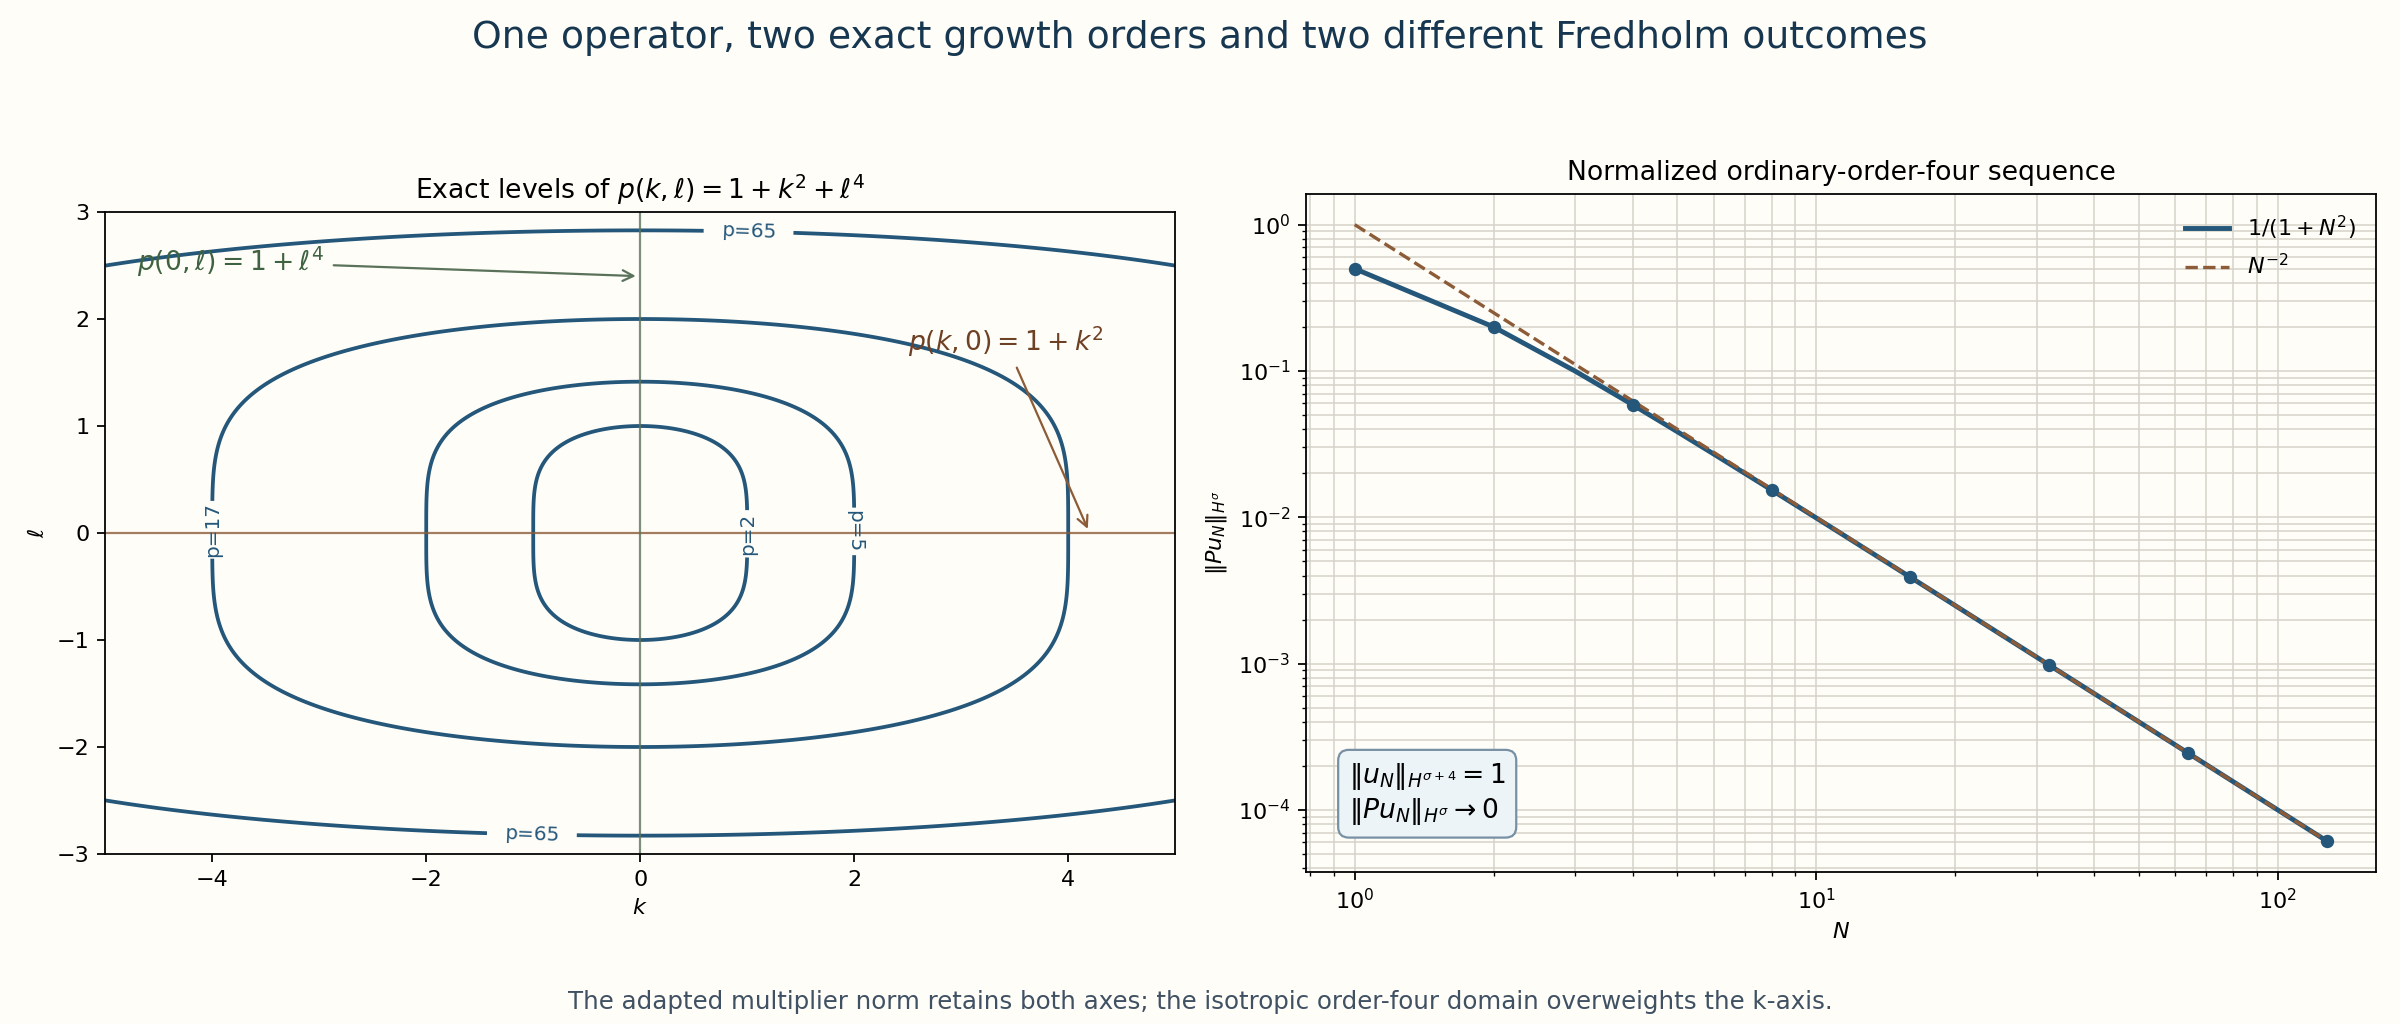
\includegraphics[keepaspectratio,alt={Exact anisotropic multiplier levels and the ordinary-scale defect sequence}]{../figures/adapted_hypoelliptic_family.png}}
\caption{Exact anisotropic multiplier levels and the ordinary-scale
defect sequence}
\end{figure}

The left panel shows the exact level sets of \(1+k^2+\ell^4\). The right
panel shows the normalized sequence that prevents the ordinary
order-four realization from having closed range. The reproducible source
is
\href{../figures/adapted_hypoelliptic_family.py}{adapted\_hypoelliptic\_family.py}.

\subsection{1. A nonelliptic operator with two exact growth
orders}\label{a-nonelliptic-operator-with-two-exact-growth-orders}

On \(\mathbb T^2=(\mathbb R/2\pi\mathbb Z)^2\), use \(D_x=-i\partial_x\)
and \(D_y=-i\partial_y\). Define \[
 P=I+D_x^2+D_y^4,\qquad
 p(k,\ell)=1+k^2+\ell^4,\qquad
 (k,\ell)\in\mathbb Z^2 .
 \tag{AH1}
\] The order-four homogeneous principal symbol is \(\eta^4\), which
vanishes at every nonzero covector \((\xi,0)\). Thus \(P\) is not
elliptic of order four. The lower-order term \(D_x^2\) is essential: it
controls the direction missed by the principal symbol.

With \(\langle k,\ell\rangle=(1+k^2+\ell^2)^{1/2}\), the complete
multiplier satisfies \[
 1+k^2+\ell^2
       \le C(1+k^2+\ell^4)
       =Cp(k,\ell)
       \le C'(1+k^2+\ell^2)^2 .
 \tag{AH2}
\] Indeed, \(\ell^2\leq1+\ell^4\) gives the first inequality, and
expanding the square gives the second. Along \((k,0)\), the multiplier
has order two. Along \((0,\ell)\), it has order four. A single isotropic
order cannot describe both axes sharply.

\subsection{2. The exact adapted domain}\label{the-exact-adapted-domain}

For \(s\in\mathbb R\), give \(H^s(\mathbb T^2)\) its Fourier norm \[
 \|f\|_{H^s}^2
 =\sum_{k,\ell\in\mathbb Z}
   \langle k,\ell\rangle^{2s}|\widehat f(k,\ell)|^2 .
\] Define the domain determined by the full operator: {\footnotesize
\[
 \mathcal D_s(P)=
 \left\{u\in\mathcal D'(\mathbb T^2):
   \sum_{k,\ell}
       \langle k,\ell\rangle^{2s}
       (1+k^2+\ell^4)^2|\widehat u(k,\ell)|^2<\infty
 \right\},
 \quad
 \|u\|_{\mathcal D_s(P)}^2
   =\sum_{k,\ell}
       \langle k,\ell\rangle^{2s}
       (1+k^2+\ell^4)^2|\widehat u(k,\ell)|^2 .
 \tag{AH3}
\]
} Multiplication of Fourier coordinates by
\(\langle k,\ell\rangle^s p(k,\ell)\) identifies this space
isometrically with \(\ell^2(\mathbb Z^2)\), so it is complete. Equation
(AH2) gives both continuous inclusions \[
 H^{s+4}(\mathbb T^2)
       \subset\mathcal D_s(P)
       \subset H^{s+2}(\mathbb T^2).
 \tag{AH4}
\] Both inclusions are strict for every \(s\). The two complete axis
sequences after (AH14) prove this, including every original weight.

For \(f\in H^s\), define the Fourier coefficients \[
 \widehat{P^{-1}f}(k,\ell)
       ={\,\widehat f(k,\ell)\over1+k^2+\ell^4}.
 \tag{AH5}
\] The denominator is positive at every lattice point. Direct
substitution gives the two exact norm identities \[
 \|P^{-1}f\|_{\mathcal D_s(P)}
       =\|f\|_{H^s},\qquad
 \|Pu\|_{H^s}
       =\|u\|_{\mathcal D_s(P)} .
 \tag{AH6}
\] The Fourier coefficients also show that \(PP^{-1}f=f\) and
\(P^{-1}Pu=u\). Therefore \[
 P:\mathcal D_s(P)\longrightarrow H^s(\mathbb T^2)
       \quad\text{is a bounded bijection with bounded inverse and index }0
       \quad\text{for every }s\in\mathbb R .
 \tag{AH7}
\]

\subsection{3. Why the ordinary order-four pair is not
Fredholm}\label{why-the-ordinary-order-four-pair-is-not-fredholm}

The map \(P:H^{s+4}\to H^s\) is bounded and injective. Let
\(u_k(x,y)=c_ke^{ikx}\), where \(c_k\) is chosen so that
\(\|u_k\|_{H^{s+4}}=1\). Then \[
 \|Pu_k\|_{H^s}
       ={1+k^2\over(1+k^2)^2}
       ={1\over1+k^2}\longrightarrow0
       \qquad (k\to\infty).
 \tag{AH8}
\] If an injective bounded operator has closed range, its inverse on
that range is bounded. That would give
\(\|Pu\|_{H^s}\geq c\|u\|_{H^{s+4}}\), contradicting (AH8). The range is
dense because every trigonometric polynomial has a finite Fourier
preimage. Section 6 below gives an element of \(H^s\) outside the range,
so the range is also proper.

\subsection{4. Hypoellipticity from the same full
multiplier}\label{hypoellipticity-from-the-same-full-multiplier}

If \(Pu\) is smooth, its Fourier coefficients decrease faster than every
power of \(\langle k,\ell\rangle\). Division by \(p(k,\ell)\geq1\)
preserves that decrease, so \(u\) is smooth. The reverse implication
follows because a differential operator maps smooth functions to smooth
functions. Hence \[
 Pu\in C^\infty(\mathbb T^2)
       \quad\Longleftrightarrow\quad
 u\in C^\infty(\mathbb T^2).
 \tag{AH9}
\] This proves global regularity and supplies the adapted Fredholm
scale. Local hypoellipticity requires a further argument, because the
Fourier coefficients in (AH9) describe the whole torus. The local kernel
proof after (AH21) supplies that argument for this operator and every
member of the family below.

\subsection{5. Every even-power anisotropic
member}\label{every-even-power-anisotropic-member}

Fix integers \(1\leq r<m\) and retain \[
 P_{r,m}=I+D_x^{2r}+D_y^{2m},\qquad
 p_{r,m}(k,\ell)=1+k^{2r}+\ell^{2m}.
 \tag{AH10}
\] Its order-\(2m\) principal symbol is \(\eta^{2m}\), so it is
nonelliptic along the nonzero covectors \((\xi,0)\).

For nonnegative \(a,b,c\), \((a+b+c)^r\leq3^{r-1}(a^r+b^r+c^r)\).
Together with \(|\ell|^{2r}\leq1+|\ell|^{2m}\), this gives \[
 \langle k,\ell\rangle^{2r}
 \leq 2\cdot3^{r-1}p_{r,m}(k,\ell).
 \tag{AH11}
\] Because \(k\) is an integer and \(r<m\), \(|k|^{2r}\leq|k|^{2m}\).
Each term in \(p_{r,m}\) is therefore bounded by
\(\langle k,\ell\rangle^{2m}\), so \[
 p_{r,m}(k,\ell)
 \leq3\langle k,\ell\rangle^{2m}.
 \tag{AH12}
\]

For \(\sigma\in\mathbb R\), define \[
 \begin{aligned}
 \mathcal D_\sigma(P_{r,m})
 =\Bigl\{u\in\mathcal D'(\mathbb T^2):
   \sum_{k,\ell\in\mathbb Z}
   \langle k,\ell\rangle^{2\sigma}
   p_{r,m}(k,\ell)^2|\widehat u(k,\ell)|^2<\infty\Bigr\},\\
 \|u\|_{\mathcal D_\sigma(P_{r,m})}^2
 =\sum_{k,\ell\in\mathbb Z}
   \langle k,\ell\rangle^{2\sigma}
   p_{r,m}(k,\ell)^2|\widehat u(k,\ell)|^2 .
 \end{aligned}
 \tag{AH13}
\] The same Fourier-coordinate isometry proves completeness. The two
full bounds give \[
 H^{\sigma+2m}(\mathbb T^2)
 \subset\mathcal D_\sigma(P_{r,m})
 \subset H^{\sigma+2r}(\mathbb T^2).
 \tag{AH14}
\] \textbf{Both inclusions are strict.} Fix any \(\sigma\in\mathbb R\).
Define two distributions by their only nonzero Fourier coefficients: \[
 \widehat u(N,0)=\langle N,0\rangle^{-\sigma-2r-1},
 \qquad
 \widehat v(0,N)=\langle0,N\rangle^{-\sigma-2r-1}
 \quad(N\geq1).
 \tag{AH22}
\] These coefficients have at most polynomial growth, so both are
distributions on the original torus. For \(u\), the full norms give \[
 \begin{aligned}
 \|u\|_{\mathcal D_\sigma(P_{r,m})}^{\,2}
 &=\sum_{N\geq1}(1+N^{2r})^2
             \langle N,0\rangle^{-4r-2}
 \leq4\sum_{N\geq1}\langle N,0\rangle^{-2}<\infty,\\
 \|u\|_{H^{\sigma+2m}}^{\,2}
 &=\sum_{N\geq1}\langle N,0\rangle^{4(m-r)-2}=\infty.
 \end{aligned}
 \tag{AH23}
\] The first estimate uses \(1+N^{2r}\leq2\langle N,0\rangle^{2r}\). For
\(v\), retaining the different multiplier on its axis gives \[
 \begin{aligned}
 \|v\|_{H^{\sigma+2r}}^{\,2}
 &=\sum_{N\geq1}\langle0,N\rangle^{-2}<\infty,\\
 \|v\|_{\mathcal D_\sigma(P_{r,m})}^{\,2}
 &=\sum_{N\geq1}(1+N^{2m})^2
                   \langle0,N\rangle^{-4r-2}\\
 &\geq 2^{-2r-1}\sum_{N\geq1}N^{4(m-r)-2}=\infty.
 \end{aligned}
 \tag{AH24}
\] Here \(1+N^{2m}\geq N^{2m}\) and \(\langle0,N\rangle\leq\sqrt2N\) for
every \(N\geq1\). Since \(m-r\geq1\), both divergent exponents are at
least \(2\). Thus \(u\) and \(v\) prove each strict inclusion in (AH14)
separately, for every \(\sigma\); \(r=1,m=2\) proves the same claim in
(AH4).

Since \(p_{r,m}\geq1\), division is defined everywhere and \[
 \widehat{P_{r,m}^{-1}f}(k,\ell)
 =\frac{\widehat f(k,\ell)}{p_{r,m}(k,\ell)},\qquad
 \|P_{r,m}^{-1}f\|_{\mathcal D_\sigma(P_{r,m})}
 =\|f\|_{H^\sigma}.
 \tag{AH15}
\] Thus \[
 P_{r,m}:\mathcal D_\sigma(P_{r,m})
 \longrightarrow H^\sigma(\mathbb T^2)
 \quad\text{is an isometric bijection of index \(0\)}
 \quad(\sigma\in\mathbb R).
 \tag{AH16}
\]

\subsection{6. Dense, proper, nonclosed ordinary
range}\label{dense-proper-nonclosed-ordinary-range}

On the ordinary pair \(P_{r,m}:H^{\sigma+2m}\to H^\sigma\), put \[
 u_N(x,y)=\langle N,0\rangle^{-\sigma-2m}e^{iNx}.
 \tag{AH17}
\] Then \(\|u_N\|_{H^{\sigma+2m}}=1\), while \[
 \|P_{r,m}u_N\|_{H^\sigma}
 =\frac{1+N^{2r}}{\langle N,0\rangle^{2m}}
 \longrightarrow0
 \qquad(N\to\infty),
 \tag{AH18}
\] The range is therefore not closed.

To prove that it is proper, define \(f\) by \[
 \widehat f(N,0)=\langle N,0\rangle^{-\sigma-1}
 \quad(N\geq1),\qquad
 \widehat f(k,\ell)=0\quad\text{otherwise}.
 \tag{AH19}
\] Then \(f\in H^\sigma\). Its unique Fourier preimage would satisfy \[
 \begin{aligned}
 \|u\|_{H^{\sigma+2m}}^2
 &=\sum_{N\geq1}
   \frac{\langle N,0\rangle^{4m-2}}
        {(1+N^{2r})^2}\\
 &\geq\frac14\sum_{N\geq1}
     N^{\,4(m-r)-2}
 =\infty .
 \end{aligned}
 \tag{AH20}
\] The inequality uses \(1+N^{2r}\leq2N^{2r}\) and
\(\langle N,0\rangle\geq N\). Since \(m-r\geq1\), the exponent is at
least \(2\). Trigonometric polynomials still lie in the range, so the
range is dense and proper.

The same rapid-decay argument proves the global equivalence: \[
 P_{r,m}u\in C^\infty(\mathbb T^2)
 \quad\Longleftrightarrow\quad
 u\in C^\infty(\mathbb T^2).
 \tag{AH21}
\]

\textbf{Local hypoellipticity, with the full inverse kernel.} For every
open \(U\subset\mathbb T^2\) and every distribution \(w\), we prove \[
 P_{r,m}w\in C^\infty(U)
       \quad\Longleftrightarrow\quad w\in C^\infty(U).
 \tag{AH25}
\] Keep the full continuous multiplier
\(p(\xi,\eta)=1+\xi^{2r}+\eta^{2m}\), put
\(q(\xi,\eta)=p(\xi,\eta)^{-1}\), and let \(\rho=r/m>0\). For a
multiindex \(\alpha=(a,b)\ne0\), repeated differentiation of the actual
reciprocal gives the finite ordered-partition formula \[
 \partial^\alpha q
 =\sum_{j=1}^{|\alpha|}(-1)^j j!\,p^{-j-1}
   \sum_{\substack{\beta_1+\cdots+\beta_j=\alpha\\|\beta_i|\geq1}}
    \frac{\alpha!}{j!\,\beta_1!\cdots\beta_j!}
    \prod_{i=1}^j\partial^{\beta_i}p .
 \tag{AH26}
\] The inner sum is over ordered nonzero multiindices. It follows by
expanding \(p(z+h)^{-1}\) to order \(|\alpha|\) using the finite Taylor
expansion of \(p(z+h)-p(z)\) in the reciprocal series: its \(j\)-th term
has sign \((-1)^j\), denominator \(p^{j+1}\), and ordered product of
\(j\) increments. The coefficient of \(h^\alpha\), multiplied by
\(\alpha!\), is exactly (AH26). Thus both factorials and every
reciprocal factor have been retained.

For \(1\leq c\leq2r\), \(\partial_\xi^c p=(2r)!/(2r-c)!\,\xi^{2r-c}\);
for \(1\leq d\leq2m\), \(\partial_\eta^d p=(2m)!/(2m-d)!\,\eta^{2m-d}\).
All mixed derivatives and derivatives beyond these two degrees are zero.
Since \(|\xi|^{2r}\leq p\) and \(|\eta|^{2m}\leq p\), each nonzero
summand in (AH26) has the bound \[
 |\partial_\xi^a\partial_\eta^b q(\xi,\eta)|
 \leq C_{a,b}\,p(\xi,\eta)^{-1-a/(2r)-b/(2m)}
 \leq C'_{a,b}\langle\xi,\eta\rangle^{-2r-a-\rho b}
 \leq C'_{a,b}\langle\xi,\eta\rangle^{-2r-\rho(a+b)} .
 \tag{AH27}
\] The same estimate for \(a=b=0\) follows directly from \(q=1/p\). The
continuous version of (AH11),
\(\langle\xi,\eta\rangle^{2r}\leq2\cdot3^{r-1}p(\xi,\eta)\), justifies
the second inequality for every real \((\xi,\eta)\). It uses
\(|\eta|^{2r}\leq1+|\eta|^{2m}\), which does not require integer
frequencies.

Let \(Q\) multiply each Fourier coefficient by
\(q(k,\ell)=(1+k^{2r}+\ell^{2m})^{-1}\). It acts on distributions and on
smooth functions because \(0<q\leq1\). Coefficientwise multiplication
proves \(QP_{r,m}=P_{r,m}Q=I\) on distributions. With ordinary Lebesgue
measure on the torus, its convolution kernel is the distribution \[
 K_Q(x,y)=(2\pi)^{-2}
       \sum_{k,\ell\in\mathbb Z}q(k,\ell)e^{i(kx+\ell y)} .
 \tag{AH28}
\] We now prove that this exact kernel is smooth away from \((0,0)\)
modulo \(2\pi\), rather than assuming that property. Define
\(\Delta_k q(k,\ell)=q(k-1,\ell)-q(k,\ell)\). The fundamental theorem of
calculus, repeated \(N\) times, gives \[
 \Delta_k^N q(k,\ell)
 =(-1)^N\int_{[0,1]^N}
       (\partial_\xi^Nq)(k-t_1-\cdots-t_N,\ell)\,dt_1\cdots dt_N .
 \tag{AH29}
\] There is the identical formula for \(\Delta_\ell^N\) with
\(\partial_\eta^Nq\) and the shift in \(\ell\). All signs and the whole
shifted reciprocal are present. For a shift of size at most \(N\), the
inequality \(\langle z\rangle\leq(1+N)\langle z-h\rangle\) shows that
(AH27) gives \[
 |\Delta_k^N q(k,\ell)|+|\Delta_\ell^N q(k,\ell)|
       \leq C_N\langle k,\ell\rangle^{-2r-\rho N}.
 \tag{AH30}
\] For each nonnegative integer \(d\), choose \(N\) so that
\(2r+\rho N>d+2\). The Fourier series with either of these difference
coefficients, and every spatial derivative of total order at most \(d\),
then converge absolutely and uniformly. Indeed, grouping the lattice
into dyadic annuli bounds the sum of \(\langle k,\ell\rangle^{-s}\),
\(s>2\), by a constant times \(\sum_{j\geq0}2^{(2-s)j}<\infty\). The
exact Fourier shift identities are \[
 \begin{aligned}
 (e^{ix}-1)^N K_Q(x,y)
   &=(2\pi)^{-2}\sum_{k,\ell}\Delta_k^Nq(k,\ell)e^{i(kx+\ell y)},\\
 (e^{iy}-1)^N K_Q(x,y)
   &=(2\pi)^{-2}\sum_{k,\ell}\Delta_\ell^Nq(k,\ell)e^{i(kx+\ell y)}.
 \end{aligned}
 \tag{AH31}
\] At every point outside the torus origin, at least one of
\(e^{ix}-1,e^{iy}-1\) is nonzero. Divide the corresponding identity by
its full smooth factor on a neighborhood of that point. The right side
is \(C^d\). Since \(d\) is arbitrary, \(K_Q\) is \(C^\infty\) off the
origin.

Suppose now that \(f=P_{r,m}w\) is smooth on \(U\). Fix an open \(V\)
with compact closure in \(U\), and choose \(\chi\in C_c^\infty(U)\)
equal to one on a neighborhood of \(\overline V\). The exact
distributional inverse gives \[
 w=Q(\chi f)+Q((1-\chi)f).
 \tag{AH32}
\] The first summand is globally smooth: \(\chi f\) is globally smooth,
its Fourier coefficients decrease rapidly, and multiplication by
\(q(k,\ell)\leq1\) preserves that decrease. In the second summand, the
support of \((1-\chi)f\) has positive distance from \(\overline V\).
Choose a smooth cutoff in the integration variable equal to one on this
support and supported away from \(\overline V\). For \(z\in V\), the
second summand is the pairing of that distribution with the cutoff times
\(K_Q(z-z')\). This is a smooth test function of \(z'\), and all its
\(z\)-derivatives are smooth and uniformly bounded on compact subsets of
\(V\), by the off-origin result above. Pairing with a distribution of
finite order therefore permits every \(z\)-derivative. The pairing
equals \(Q((1-\chi)f)\): approximate \((1-\chi)f\) by convolution with
smooth approximate identities of shrinking support; the separated kernel
pairings converge with all derivatives on compact subsets of \(V\),
while Fourier multiplication by \(q\) converges distributionally to the
exact second summand. It follows that both summands in (AH32) are smooth
on \(V\). Such sets \(V\) cover \(U\). The reverse implication in (AH25)
follows from locality of the differential operator. This proves local
hypoellipticity for every \(1\leq r<m\), including the original
\(I+D_x^2+D_y^4\), without changing any adapted norm or multiplier.

\begin{figure}
\centering
\pandocbounded{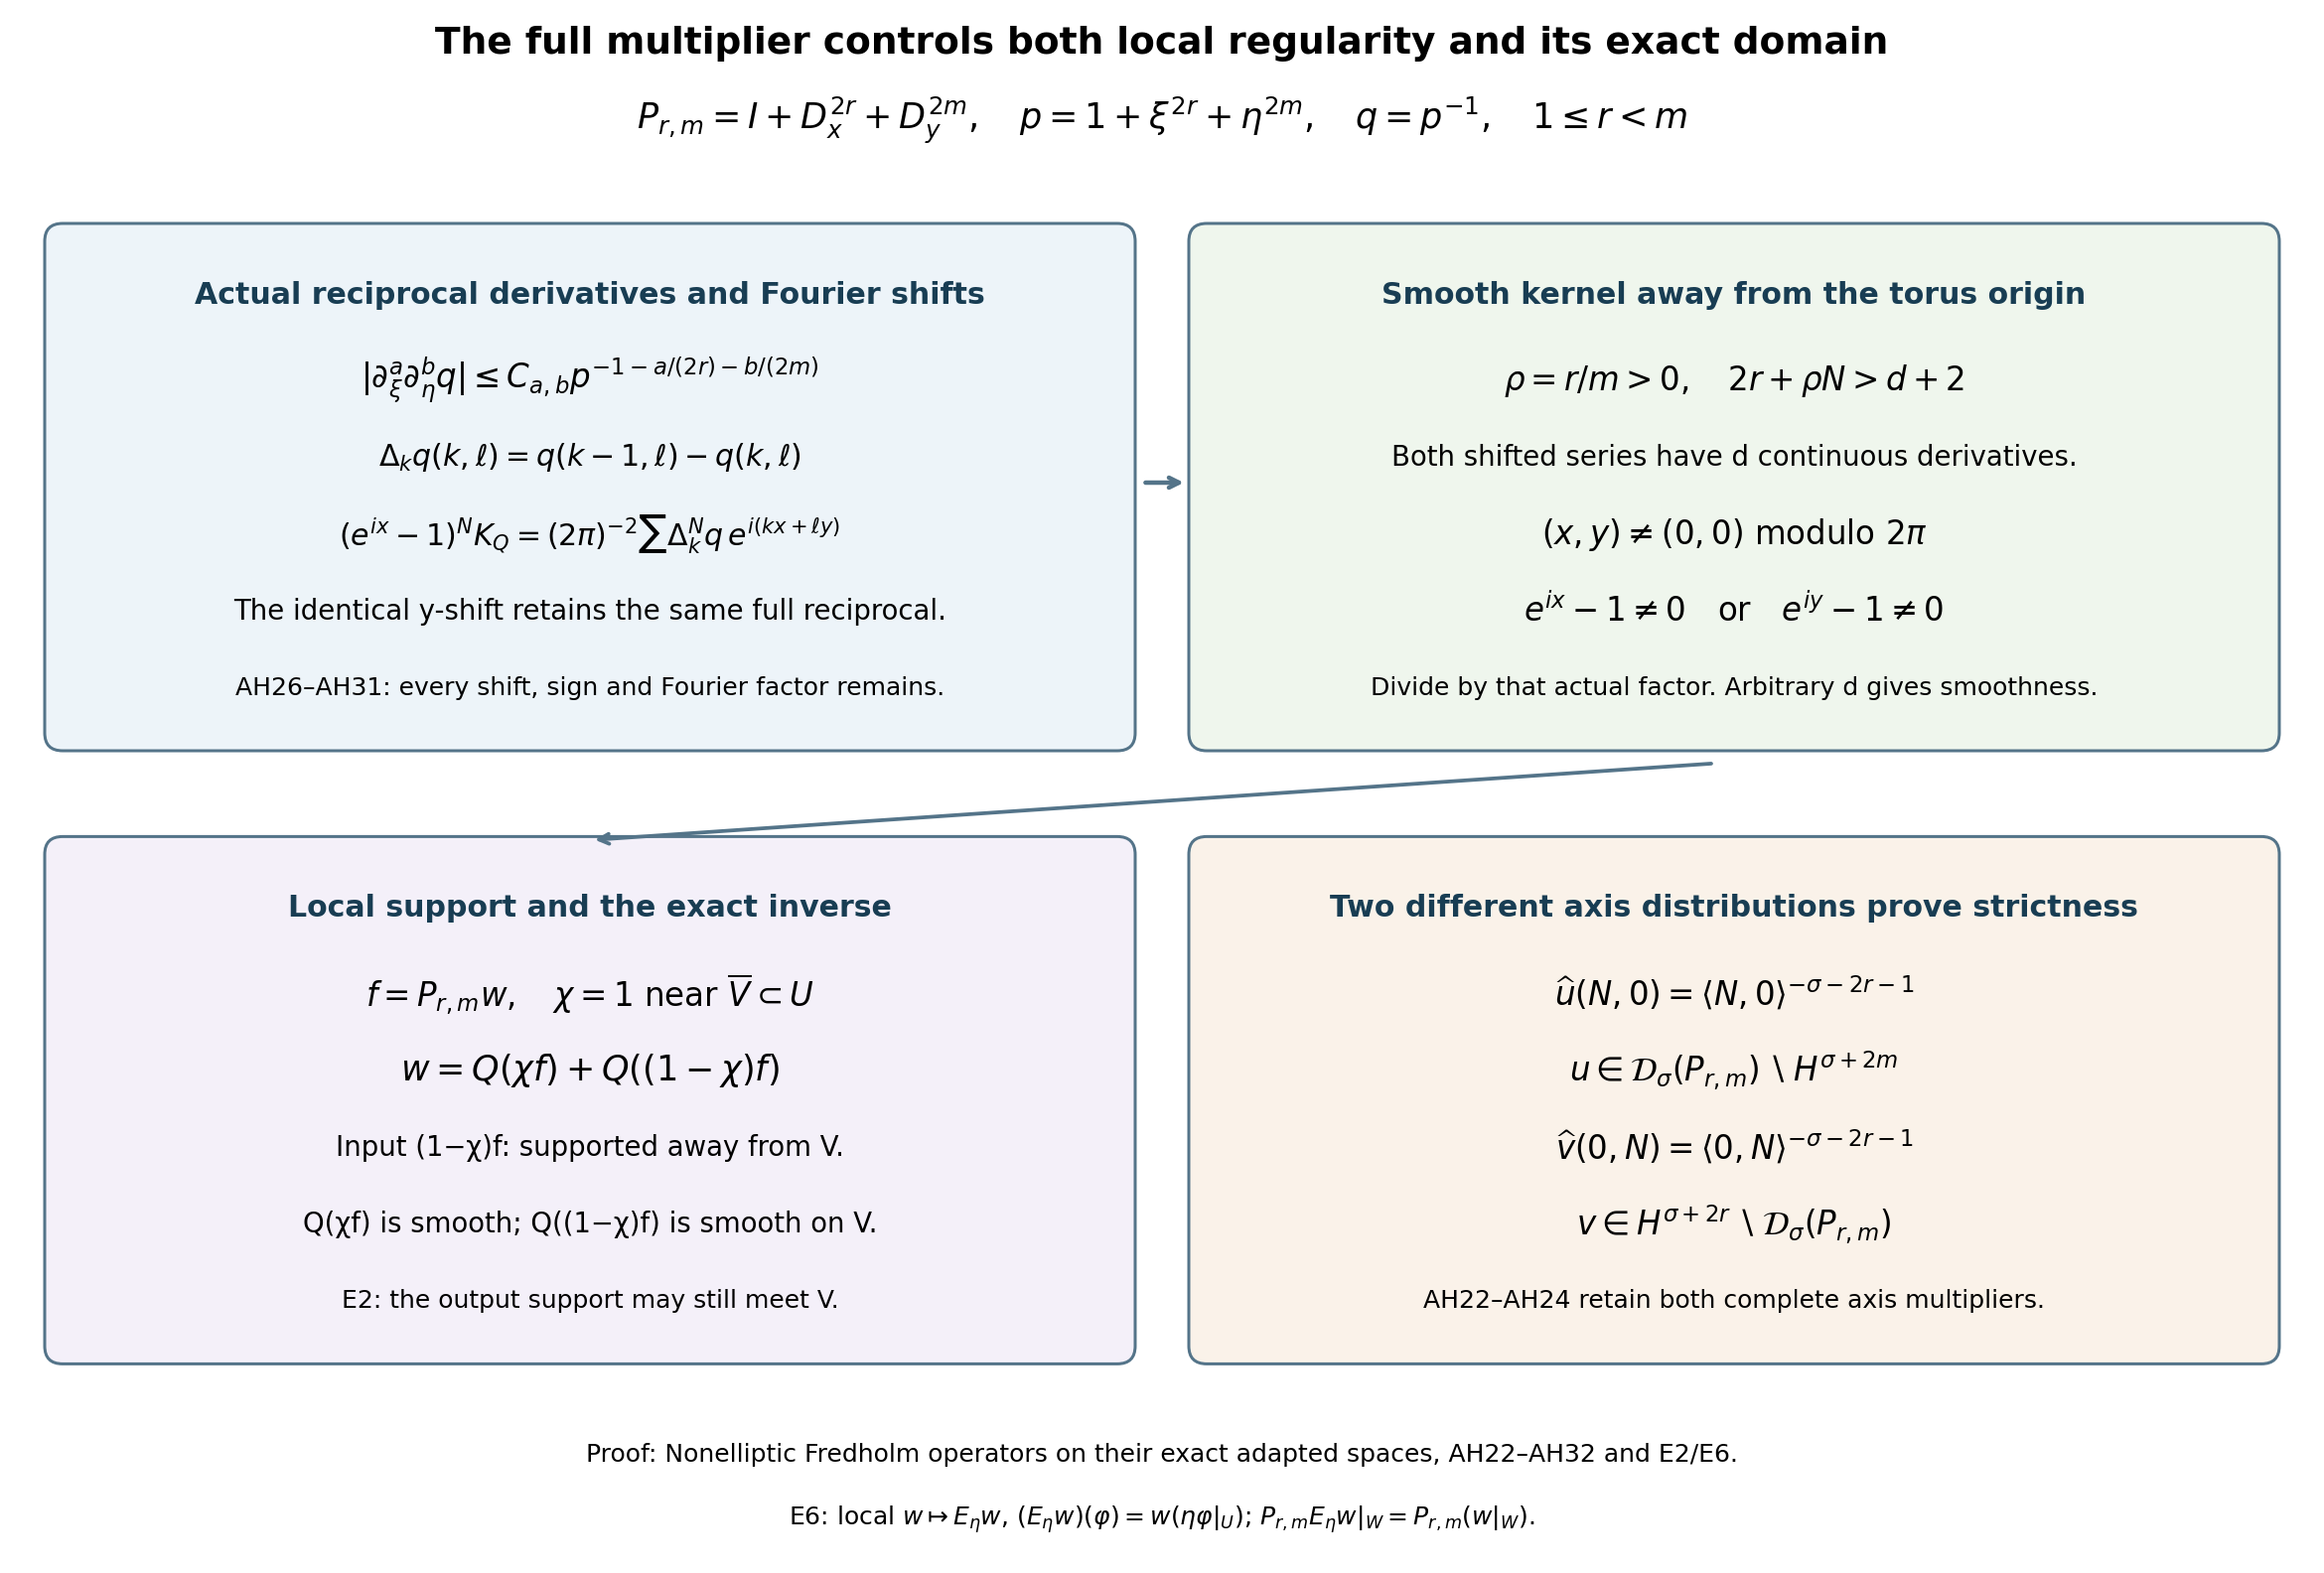
\includegraphics[keepaspectratio,alt={The original inverse kernel and the two strict axis inclusions}]{../figures/adapted-local-kernel.png}}
\caption{The original inverse kernel and the two strict axis inclusions}
\end{figure}

The diagram records the exact reciprocal, its two Fourier difference
identities, the separated support in (AH32), and the two actual
distributions proving strictness in (AH22)--(AH24). The proofs are
(AH25)--(AH32) and (AH22)--(AH24). The reproducible source is
\href{../figures/adapted-local-kernel.py}{adapted-local-kernel.py}.

\subsection{7. Worked member: orders four and
six}\label{worked-member-orders-four-and-six}

Take \(r=2\) and \(m=3\). Then \[
 P_{2,3}=I+D_x^4+D_y^6,\qquad
 H^{\sigma+6}\subset\mathcal D_\sigma(P_{2,3})
 \subset H^{\sigma+4}.
 \tag{AF1}
\] On the normalized \(k\)-axis sequence, the ordinary order-six output
is \[
 \|P_{2,3}u_N\|_{H^\sigma}
 =\frac{1+N^4}{(1+N^2)^3}
 \longrightarrow0 .
 \tag{AF2}
\] The same operator is therefore an isometric bijection on its adapted
domain and non-Fredholm on the ordinary order-six pair.

\subsection{8. Exercises with solutions}\label{exercises-with-solutions}

\textbf{Exercise 1.} For \(P_{1,3}=I+D_x^2+D_y^6\), state the two
Sobolev spaces that bound its adapted domain and compute the decay power
of the normalized ordinary order-six sequence.

\textbf{Solution.} Equations (AH11)--(AH14) give \[
 H^{\sigma+6}\subset\mathcal D_\sigma(P_{1,3})
 \subset H^{\sigma+2}.
\] Along the \(k\)-axis, \[
 \frac{1+N^2}{(1+N^2)^3}
 =\frac1{(1+N^2)^2}\sim N^{-4}.
\]

\textbf{Exercise 2.} Compare the adapted norm with the usual graph norm
\(\|u\|_{H^\sigma}+\|P_{r,m}u\|_{H^\sigma}\).

\textbf{Solution.} Since \(p_{r,m}\geq1\), \[
 \|u\|_{H^\sigma}
 \leq\|P_{r,m}u\|_{H^\sigma}
 =\|u\|_{\mathcal D_\sigma(P_{r,m})}.
\] Consequently \[
 \|u\|_{\mathcal D_\sigma(P_{r,m})}
 \leq\|u\|_{H^\sigma}+\|P_{r,m}u\|_{H^\sigma}
 \leq2\|u\|_{\mathcal D_\sigma(P_{r,m})}.
\] The adapted norm is exactly the output norm and is equivalent to the
full graph norm with the displayed constants.

\subsection{References}\label{references}

The theorem proved here is the explicit \(P_{r,m}\)-family above; it
does not state that every operator in those broader classes has been
reduced to this Fourier model.

\subsection{Editorial supplement: the original torus inverse, exact
domains and sharp consequences}\label{AN03-U043-COMPLETE}

\emph{Editorial proof completed in October 2026; CC0.}

This supplement supplies the Fourier and distribution receivers of
(AH3), (AH13) and (AH25)--(AH32), and proves further consequences for
the same operators. Equations (AH1)--(AH32), their original order, both
worked solutions and (AF1)--(AF2) above remain unchanged. Throughout,
\(1\leq r<m\) are integers, \(\sigma\in\mathbb R\), the torus has period
\(2\pi\) in each coordinate, and \(p(k,\ell)=1+k^{2r}+\ell^{2m}\). Every
norm below is the original Fourier norm. The weighted Euclidean norms in
\href{mixed-sobolev-mapping.pdf}{the earlier Sobolev lesson,
(MSB3)--(MSB5)} explain the preceding reading link; the torus statement
and its measure factor are proved here. No general nonelliptic Fredholm
theorem is needed. The scalar and finite-coordinate derivative, Taylor
and real-power rules are proved in
\href{metric-foundation-bridges.pdf\#section*.74}{the
metric foundation, Sections 13.1--13.8}. The integrations and linear
substitutions below use
\href{banach-foundation-bridges.pdf\#section*.83}{the
Banach foundation, (LP1)--(LP5)}, restricted to the original torus
coordinate box when the domain is compact. They supply absolutely
integrable Fubini and the complete translation and scaling Jacobians;
the only nonnegative infinite sums below are increasing limits of finite
sums. The torus boundary faces have Lebesgue measure zero by that
foundation's full box-volume argument.

\subsubsection{E1. The torus Fourier and distribution
maps}\label{e1.-the-torus-fourier-and-distribution-maps}

Put \(z=(x,y)\), \(\kappa=(k,\ell)\), and
\(\langle\kappa\rangle=(1+k^2+\ell^2)^{1/2}\). Use complex-linear
distribution pairing and ordinary Lebesgue measure, with the exact
convention \[
 \widehat f(\kappa)=(2\pi)^{-2}\int_{[0,2\pi]^2}
       f(z)e^{-i\kappa\cdot z}\,dz,
 \qquad
 \widehat T(\kappa)=(2\pi)^{-2}T(e^{-i\kappa\cdot z}).
 \tag{AE1}
\] The period, derivatives and complete orthogonality integrals of these
characters are proved in
\href{metric-foundation-bridges.pdf\#section*.122}{the
metric foundation, (OC33)--(OC37)}, including the original zero-mode
integral \(2\pi\). In particular its addition laws give
\(|1-e^{it}|^2=4\sin^2(t/2)\), the precise factor used in the finite
geometric estimate below. Boundary integration by parts has no boundary
term for periodic smooth functions. For every integer \(L\geq0\),
\(\langle\kappa\rangle^{2L}\widehat f(\kappa)
=\widehat{(I-\partial_x^2-\partial_y^2)^L f}(\kappa)\). Thus smooth
functions have rapidly decreasing coefficients. Conversely, if for every
\(M\) the coefficients \(c_\kappa\) satisfy
\(\sup_\kappa\langle\kappa\rangle^M|c_\kappa|<\infty\), the series
\(\sum c_\kappa e^{i\kappa\cdot z}\), and each differentiated series,
converge absolutely and uniformly. To verify summability, a dyadic shell
\(2^j\leq\langle\kappa\rangle<2^{j+1}\) contains at most
\((2\lceil2^{j+1}\rceil+1)^2\leq25\,2^{2j+2}\) points. Consequently
\(\sum\langle\kappa\rangle^{-s}<\infty\) for \(s>2\). Repeated
integration of the uniformly convergent derivative series proves that
their sum is smooth and has precisely the specified coefficients.

Here is also the required uniqueness, rather than an assumption that the
characters are complete. For \(N\geq0\), define the finite trigonometric
polynomial \[
 F_N(t)=\frac1{N+1}\left|\sum_{j=0}^N e^{ijt}\right|^2
  =\sum_{|a|\leq N}\left(1-\frac{|a|}{N+1}\right)e^{iat}.
 \tag{AE2}
\] The second identity follows by counting the ordered pairs of indices
whose difference is \(a\). Thus \(F_N\geq0\) and
\(\int_0^{2\pi}F_N(t)\,dt=2\pi\). Away from zero modulo \(2\pi\), the
finite geometric sum gives \(F_N(t)\leq[(N+1)\sin^2(t/2)]^{-1}\).
Therefore the ordinary Lebesgue convolution kernel
\(J_N(x,y)=(2\pi)^{-2}F_N(x)F_N(y)\) has mass one and its mass outside
any fixed neighborhood of the torus origin tends to zero. For a
continuous function, split \(J_N*f-f=\int J_N(v)(f(z-v)-f(z))\,dv\) into
that neighborhood and its complement. Uniform continuity bounds the
first part by its modulus of continuity; the second part is bounded by
\(2\|f\|_\infty\) times the mass just estimated. This proves uniform
convergence. For smooth functions the same proof applied to each
derivative proves convergence in every smooth seminorm, since
differentiation commutes with convolution with this finite polynomial. A
continuous function with all Fourier coefficients zero consequently
vanishes. Applying this to the difference of a smooth function and its
absolutely convergent Fourier series proves its reconstruction,
including all derivatives.

On the compact torus a distribution means a continuous linear functional
on \(C^\infty\), whose defining seminorms are
\(\max_{|\alpha|\leq N}\|\partial^\alpha\phi\|_\infty\). Continuity at
zero gives one integer \(N\) and a constant \(C\) such that \[
 |T(\phi)|\leq C\max_{|\alpha|\leq N}
                    \|\partial^\alpha\phi\|_\infty.
 \tag{AE3}
\] Indeed, a finite intersection of seminorm balls lies in the inverse
image of the unit disk; replace their orders by their maximum and scale
the test function. Testing exponentials proves polynomial growth of
\(\widehat T\). Conversely, if
\(|c_\kappa|\leq C\langle\kappa\rangle^A\), define \[
 T_c(\phi)=(2\pi)^2\sum_{\kappa\in\mathbb Z^2}
                        c_\kappa\widehat\phi(-\kappa).
 \tag{AE4}
\] Choose an integer \(L\) with \(2L>A+2\). The integration-by-parts
bound above proves absolute convergence and bounds (AE4) by a constant
times the supremum norms of derivatives of \(\phi\) through order
\(2L\). Thus it is a distribution, and direct testing in (AE1) gives
\(\widehat{T_c}=c\). Finally, the smooth reconstruction of \(\phi\)
converges in every seminorm, so every distribution applied to that
reconstruction equals (AE4) with its own coefficients. This proves
distributional uniqueness and all the maps just used.

In particular, if \(a\in\ell^2(\mathbb Z^2)\), both
\(\langle\kappa\rangle^{-\sigma}a_\kappa\) and
\(\langle\kappa\rangle^{-\sigma}p(\kappa)^{-1}a_\kappa\) have polynomial
growth: \(|a_\kappa|\leq\|a\|_2\) and \(p^{-1}\leq1\). Equation (AE4)
proves that they really define distributions. The two coordinate maps \[
 H^\sigma\longrightarrow\ell^2,\quad
 f\longmapsto(\langle\kappa\rangle^\sigma\widehat f(\kappa))_\kappa,
 \qquad
 \mathcal D_\sigma(P_{r,m})\longrightarrow\ell^2,\quad
 u\longmapsto(\langle\kappa\rangle^\sigma p(\kappa)
                                      \widehat u(\kappa))_\kappa
 \tag{AE5}
\] are therefore onto isometries, with the displayed inverse coefficient
maps. Enumerate the origin first, then each finite square shell
\(\max(|k|,|\ell|)=j\), \(j=1,2,\ldots\), in lexicographic order. This
is an explicit bijection \(\mathbb N\to\mathbb Z^2\), and pullback of
coordinates preserves every nonnegative squared sum. Completeness of
\(\ell^2\), proved in
\href{banach-foundation-bridges.pdf\#section*.26}{the
Banach foundation, Section 11}, proves both completeness assertions;
coordinate truncations prove density of finite Fourier polynomials in
both spaces. The same bounds show that norm convergence there implies
distributional convergence. Orthogonality of the characters, integrated
with ordinary Lebesgue measure, gives for every finite polynomial \(f\)
\(\|f\|_{H^0}^2=(2\pi)^{-2}\int|f|^2\). An \(H^0\)-Cauchy polynomial
sequence has an ordinary \(L^2\) limit by
\href{banach-foundation-bridges.pdf\#section*.94}{the
Banach foundation, Section 15.3}. Testing against a smooth function and
Cauchy--Schwarz identifies that limit with the distribution supplied by
(AE4). Passing the finite norm identity to the limit retains precisely
the factor \((2\pi)^{-2}\).

Since differentiation multiplies the coefficients by \(k^{2r}\) or
\(\ell^{2m}\), (AE5) proves the actual maps, both inverse products and
every norm identity in (AH5)--(AH7) and (AH15)--(AH16). Their kernels
and cokernels are zero and their ranges are the entire Banach target, so
the index is zero in the definition of
\href{fredholm-stability.pdf\#section*.2}{the
Fredholm lesson, (F1)}. The power inequality preceding (AH11) follows
from convexity of \(t\mapsto t^r\), or directly its nonnegative second
derivative for \(r\geq2\) and equality for \(r=1\). Its continuous
version uses \(|\eta|^{2r}\leq1+|\eta|^{2m}\); the lattice version of
(AH12) uses \(|k|^{2r}\leq|k|^{2m}\). Thus their stated constants and
all the inclusions are valid. Equations (AH22)--(AH24), now genuine
distributions by (AE4), establish their stated strictness. The same
construction proves the existence of (AH19), whose squared norm is
\(\sum_{N\geq1}(1+N^2)^{-1}<\infty\). Its preimage is excluded by the
complete calculation (AH20), while polynomial density proves density of
the ordinary range. A dense proper linear subspace is not closed.
Alternatively the closed-range inverse assertion used in (AH8) follows
by applying
\href{banach-foundation-bridges.pdf\#section*.19}{the
proved bounded inverse theorem, (B8)--(B9)} to the injective map onto
its closed Banach range. Its lower bound contradicts the exact sequence
(AH18). This supplies both arguments at every real \(\sigma\). Rapid
decay and multiplication by the original polynomial prove (AH9) and
(AH21) in both directions.

\subsubsection{E2. The full local kernel and the separated distribution
pairing}\label{e2.-the-full-local-kernel-and-the-separated-distribution-pairing}

The finite expansion used in (AH26) can be justified without any formal
infinite series. At a fixed \(z=(\xi,\eta)\), put \(b(h)=p(z+h)-p(z)\).
For small \(h\), \(|b(h)|<p(z)/2\), and the finite geometric identity
with remainder gives \[
 \frac1{p(z)+b(h)}
 =\sum_{j=0}^{L}(-1)^j p(z)^{-j-1}b(h)^j
  +\frac{(-1)^{L+1}b(h)^{L+1}}
              {p(z)^{L+1}(p(z)+b(h))}.
 \tag{AE6}
\] Take \(L=|\alpha|\). Since \(b(0)=0\), every derivative of the
remainder through order \(L\) at zero is zero, by the finite Leibniz
rule. Expanding each increment by its actual polynomial Taylor formula
and differentiating the coefficient of \(h^\alpha\) proves exactly the
ordered sum (AH26), with both \(j!\) factors retained. A nonzero
derivative factor is a pure \(\xi\)- or pure \(\eta\)-derivative, and
its exact factorial gives respectively a bound \(C p^{1-c/(2r)}\) or
\(C p^{1-d/(2m)}\). Multiplying the \(j\) factors in their given order
and the actual \(p^{-j-1}\) gives the first estimate (AH27). Raising the
continuous lower bound (AH11) to the positive power \(1+a/(2r)+b/(2m)\)
gives its second estimate with exponent \(-2r-a-(r/m)b\). Since
\(0<\rho=r/m<1\), the third estimate follows with every exponent as
written. The zero multiindex is covered by the direct reciprocal.

Polynomial-growth and rapid-decay sequences in E1 show that
multiplication by \(q\) defines \(Q\) on distributions and on smooth
functions; the latter map is continuous in the smooth topology. Indeed
the integration-by-parts estimate and the summability bound in E1 bound
each output derivative seminorm by finitely many input derivative
seminorms. The even identity \(q(-\kappa)=q(\kappa)\) gives
\((QT)(\phi)=T(Q\phi)\) under the complex-linear convention.
Consequently distributional convergence of \(T_j\) implies that of
\(QT_j\). Their exact coefficient products are one for \(QP_{r,m}\) and
\(P_{r,m}Q\).

The ordinary convolution of smooth functions has Fourier coefficients
\((2\pi)^2\widehat f(\kappa)\widehat g(\kappa)\): substitute \(z=z'+v\)
in its defining integral. The coefficients of (AH28) are
\((2\pi)^{-2}q(\kappa)\), so its convolution with a smooth function has
exactly coefficients \(q(\kappa)\widehat f(\kappa)\). Equivalently,
distributional convolution with a smooth function is the pairing with
its translated smooth test function; (AE4) gives the same coefficients.
This proves the kernel formula with its ordinary measure.

For completeness, the Fourier coefficient of \(e^{ix}K_Q\) at
\((k,\ell)\) is \((2\pi)^{-2}q(k-1,\ell)\), so iteration of the actual
difference proves both identities (AH31) as distributions. The repeated
fundamental theorem of calculus proves (AH29), including \((-1)^N\) and
the entire shift. For \(|h|\leq N\), the triangle inequality in
\(\mathbb R^3\) applied to \((1,z-h)+(0,h)\) gives
\(\langle z\rangle\leq(1+N)\langle z-h\rangle\). This proves (AH30). For
any requested derivative order \(d\), choose an integer \(N\) with
\(2r+\rho N>d+2\). The explicit lattice summability bound in E1 makes
both right sides of (AH31) \(C^d\). Division by the specified nonzero
smooth factor works on its own neighborhood. These distributional
representatives agree on overlaps because distributional reconstruction
is unique. Taking arbitrary \(d\) therefore proves that the original
\(K_Q\) is smooth off the torus origin, with no choice of an alternative
inverse kernel.

We now verify the cutoff and limiting operations in (AH32). The smooth
cutoffs used here are supplied by the explicit compact bump construction
in
\href{metric-foundation-bridges.pdf\#section*.128}{the
metric foundation, Section 13.10, (OC38)--(OC41)}. For a compact set
contained in an open set on the torus, cover it by finitely many
coordinate balls whose closures lie in that open set. On each ball the
Euclidean bump construction gives \(0\leq\chi_j\leq1\), equal to one on
a smaller ball, and supported inside the original ball; extension by
zero is smooth. The finite expression \(1-\prod_j(1-\chi_j)\) is the
desired cutoff, equal to one on a neighborhood of the compact set. This
proves the stated torus cutoff receiver, including the case of the whole
torus.

The distance here is the original flat quotient distance
\(d(z,z')=\min_{a\in\mathbb Z^2}|z-z'+2\pi a|\). The minimum is
attained: for representatives in \([0,2\pi]^2\), the zero shift already
gives a fixed finite upper bound, so all larger shifts can be excluded
and only finitely many remain. The triangle inequality follows by adding
the minimizing shifts, and distance varies continuously by that
inequality. The torus is compact, being the continuous image of the
original compact square. Thus two disjoint compact sets have a positive
minimum distance: distance attains a minimum on their compact product,
and a zero minimum would give a common point. This supplies the exact
support separation used next. Every point of an open \(U\) has a small
metric ball \(V\) with compact closure in \(U\), by taking half the
radius of a ball contained in \(U\); such \(V\) cover \(U\). For empty
\(U\), both local assertions are vacuous.

Set \(g=(1-\chi)f\) with \(f=P_{r,m}w\) and the original \(\chi=1\) near
\(\overline V\). Its support \(S\) is a compact set disjoint from a
neighborhood of \(\overline V\), hence has positive distance from
\(\overline V\) if it is nonempty. Choose by the preceding construction
a cutoff \(\zeta\) equal to one on a neighborhood of \(S\) and with
support a positive distance from \(\overline V\). If \(g=0\), the second
term is zero and there is nothing to pair. Otherwise, for \(z\in V\),
the function \[
 F(z)=g\bigl(z'\longmapsto\zeta(z')K_Q(z-z')\bigr)
 \tag{AE7}
\] is well defined. The test function in (AE7) is globally smooth in
\(z'\), since its cutoff is zero near the possible singularity \(z'=z\).
All its mixed \(z,z'\) derivatives are bounded when \(z\) ranges over a
compact subset of \(V\). Taylor's formula with uniform derivative
remainders in the \(z'\) seminorm of (AE3) proves that difference
quotients of (AE7) converge to the pairing with the corresponding
\(z\)-derivative. Repeating this proves \(F\in C^\infty(V)\).

To identify this particular pairing with the actual \(Qg\), choose a
nonnegative \(\theta\in C_c^\infty(\mathbb R^2)\), supported in the unit
ball, with \(\int\theta=1\). The bump just described divided by its
positive integral gives such a function, retaining that integral in the
normalization. For \(h>0\), periodize its original scaling: \[
 \theta_h(z)=h^{-2}\sum_{a\in\mathbb Z^2}
                     \theta\bigl((z+2\pi a)/h\bigr),
 \qquad
 \widehat{\theta_h}(\kappa)
   =(2\pi)^{-2}\int_{\mathbb R^2}
                   \theta(v)e^{-ih\kappa\cdot v}\,dv.
 \tag{AE8}
\] The sums are locally finite. Substitution \(z+2\pi a=hv\), with
Jacobian \(h^2\), proves mass one on the original torus and the
displayed coefficient. The convolution \(g_h=\theta_h*g\) is smooth,
since it is the distribution pairing with a jointly smooth kernel. Its
support is contained in the torus \(h\)-neighborhood of \(S\). Testing
convolution against a smooth function amounts to convolving that test
function with the reflected \(\theta_h\); the mean-value bound for every
derivative proves convergence to that test function in \(C^\infty\). By
(AE3), \(g_h\to g\) distributionally. Its Fourier multiplier is the full
integral on the right of (AE8), since the convolution coefficient
\((2\pi)^2\) cancels the explicitly displayed \((2\pi)^{-2}\); the
integral is bounded by one and tends to one.

For sufficiently small \(h\), \(\zeta=1\) on \(\operatorname{supp}g_h\).
Convolution of \(K_Q\) with the smooth \(g_h\), already identified by
its exact coefficients, can then be restricted to the region away from
the singularity for \(z\in V\). It equals \(g_h(\zeta(z')K_Q(z-z'))\)
there, with ordinary measure and no extra factor. This can also be
checked by testing in \(z\) with a compactly supported smooth function
in \(V\): the distributional kernel is paired only against tests
supported away from its origin and therefore equals its established
smooth representative there. As \(h\downarrow0\), all derivatives of
these pairings converge uniformly on compact subsets of \(V\) to those
of (AE7). Indeed, reflected convolution converges uniformly in every
\(z'\) seminorm on the compact family of joint derivatives of
\(\zeta(z')K_Q(z-z')\), and (AE3) bounds the errors. On the other hand
\(Qg_h\to Qg\) distributionally by the proved transpose formula for
\(Q\). Thus (AE7) is exactly the restriction of \(Qg\) to \(V\). The
first term in (AH32) is globally smooth, since \(\chi f\) extends
smoothly by zero and has rapidly decreasing coefficients. This proves
the forward direction of (AH25) on every such \(V\), hence on \(U\). The
reverse direction follows from the local derivatives defining
\(P_{r,m}\), so all of (AH25) is proved.

An editorial clarification to the existing diagram is needed: the
sentence ``Second term: its support stays away from V'' in
\(\texttt{adapted-local-kernel.png}\) refers to the input distribution
\((1-\chi)f\). The support of its output \(Q((1-\chi)f)\) need not stay
away from \(V\). The exact assertion proved by (AE7)--(AE8) is that this
output is smooth on \(V\). This identifies the support ambiguity while
retaining the original diagram and its reproducible source. There is an
explicit counterexample to interpreting it as a support assertion about
the output. Choose a small coordinate rectangle and an open \(V\) with
closure inside it, containing the chart origin. Put
\(v_r(x)=\sum_{j\geq0}(-1)^{(r+1)j}x^{2rj}/(2rj)!\). The factorial bound
makes this series and every derivative uniformly convergent on compact
intervals; shifting its index proves \(v_r^{(2r)}=(-1)^{r+1}v_r\). Since
\(v_r(0)=1\), choose the rectangle small enough that \(v_r\ne0\) there,
and a smooth cutoff \(\eta\) supported in that rectangle and equal to
one on a neighborhood of \(\overline V\). The globally smooth function
\(u(z)=\eta(z)v_r(x)\), extended by zero, satisfies \(Pu=0\) where
\(\eta=1\), since \((-1)^r\partial_x^{2r}v_r=-v_r\) and its
\(y\)-derivative there is zero. Choose the original-type \(\chi=1\) near
\(\overline V\) supported within that neighborhood. For \(f=Pu\), one
has \(\chi f=0\), hence \(g=(1-\chi)f=f\) and \(Qg=QPu=u\), which is
nonzero on \(V\). Its input support is separated from \(V\), and its
output is smooth and nonzero there. More generally (AE7) is the exact
linear map from distributions supported in \(S\) to smooth functions on
\(V\). For a distribution satisfying (AE3) with order \(N\), its
derivative of order \(\alpha\) is bounded on any compact \(L\subset V\)
by \(C\max_{|\beta|\leq N}\sup_{z\in L,z'}
|\partial_z^\alpha\partial_{z'}^\beta
(\zeta(z')K_Q(z-z'))|\). Thus the actual support defect gives a proved
smooth receiving map rather than a false support-preserving assertion.
The continuous level curves in the first existing figure are the
continuous \((k,\ell)\)-section of the same full polynomial; the actual
Fourier indices of the operator remain the lattice \(\mathbb Z^2\).

\subsubsection{E3. Exact derivative domains and the unbounded
realization}\label{e3.-exact-derivative-domains-and-the-unbounded-realization}

There is an additional exact domain description, with its original norm
retained: \[
 \mathcal D_\sigma(P_{r,m})
 =\{u\in H^\sigma:D_x^{2r}u\in H^\sigma,
                         \ D_y^{2m}u\in H^\sigma\}.
 \tag{AE9}
\] The arrows in this equality are identity maps on distributions. To
prove both directions and their norm bounds, set
\(A_\sigma(u)=\|u\|_{H^\sigma}^2+
\|D_x^{2r}u\|_{H^\sigma}^2+\|D_y^{2m}u\|_{H^\sigma}^2\). The full
expansion and finite Cauchy--Schwarz inequality give \[
 \begin{split}
 p(k,\ell)^2
  &=1+k^{4r}+\ell^{4m}+2k^{2r}+2\ell^{2m}
                                         +2k^{2r}\ell^{2m},\\
 A_\sigma(u)&\leq\|u\|_{\mathcal D_\sigma(P_{r,m})}^2
                                      \leq3A_\sigma(u).
 \end{split}
 \tag{AE10}
\] The inequalities hold first term by term, then after summing
nonnegative terms, including infinite sums. They prove (AE9), its
bounded inverse identity maps and the presence of every original
cross-term. The graph norm comparison in Exercise 2 follows
independently from \(\|u\|_{H^\sigma}\leq\|Pu\|_{H^\sigma}
=\|u\|_{\mathcal D_\sigma}\), with its exact constants one and two.

Regard the same differential operator as an unbounded operator on the
original \(H^\sigma\). Its maximal domain
\(\{u\in H^\sigma:Pu\in H^\sigma\}\) is exactly (AH13): coefficientwise
this condition is
\((\langle\kappa\rangle^\sigma p\widehat u)_\kappa\in\ell^2\), and
\(p\geq1\) ensures the required input membership. It is densely defined,
closed, positive and selfadjoint. These assertions can all be verified
on the exact orthonormal basis \[
 e_{\kappa,\sigma}(z)=\langle\kappa\rangle^{-\sigma}
                                      e^{i\kappa\cdot z},
 \qquad P e_{\kappa,\sigma}=p(\kappa)e_{\kappa,\sigma}.
 \tag{AE11}
\] Density follows from E1. If \(u_j\to u\) and \(Pu_j\to v\) in
\(H^\sigma\), each coefficient converges, giving
\(p\widehat u=\widehat v\). The maximal-domain condition then proves
closedness and \(Pu=v\). For \(u\) in this domain,
\(\langle Pu,u\rangle_{H^\sigma}
=\sum_\kappa p(\kappa)|\langle\kappa\rangle^\sigma
\widehat u(\kappa)|^2\geq\|u\|_{H^\sigma}^2\), with convergence by
Cauchy--Schwarz. The same coefficient calculation proves symmetry. If a
vector \(v\) is in the adjoint domain, testing against every basis
vector in (AE11) forces the coefficients of its adjoint image to be
\(p\) times those of \(v\). Square summability of that image is exactly
the maximal-domain condition. Conversely that condition makes the
symmetry identity valid for every input by Cauchy--Schwarz, and hence
puts \(v\) in the adjoint domain. This proves selfadjointness, without
an imported unbounded spectral theorem. Finite Fourier truncations
converge in both input and output norms, so these polynomials form a
graph core for this actual realization.

Its inverse on \(H^\sigma\) is the same full \(Q\). Its norm is one,
attained at the origin frequency; it is positive and compact. For
compactness, truncate to \(|\kappa|\leq R\). The operator-norm error is
\(\sup_{|\kappa|>R}p(\kappa)^{-1}\to0\), by (AH11). Finite-rank maps are
compact, and an operator-norm limit of them is compact: for a prescribed
error choose a truncation with smaller norm error and a finite net of
its bounded image; this gives a finite net of the full image. For any
sequence in its closure, successive finite nets of radii \(2^{-j}\)
allow nested subsequences contained in a single net ball at each stage;
the diagonal subsequence is Cauchy. Completeness gives its limit in that
closed set. The metric compactness equivalence proved in
\href{banach-foundation-bridges.pdf\#section*.23}{the
Banach foundation, Section 10} then proves compactness.

The spectrum of the unbounded realization is exactly the set of numbers
\(1+k^{2r}+\ell^{2m}\), with each original lattice multiplicity. Every
such number has its basis eigenvectors. If \(\lambda\) is not in that
set, the set has only finitely many elements in each bounded interval,
because \(p\leq R\) bounds both \(|k|\) and \(|\ell|\). It follows that
\(\inf_\kappa|p(\kappa)-\lambda|>0\) and
\(\sup_\kappa p(\kappa)/|p(\kappa)-\lambda|<\infty\). The coefficient
map \(f\mapsto\widehat f/(p-\lambda)\) is therefore bounded from
\(H^\sigma\) into the exact domain (AH13), and verifies both inverse
products for \(P-\lambda\). It is in particular a bounded inverse into
\(H^\sigma\); this proves the claimed spectrum with the original
domains.

\subsubsection{E4. Sharp isotropic gain, compact embeddings and every
bounded ordinary
pair}\label{e4.-sharp-isotropic-gain-compact-embeddings-and-every-bounded-ordinary-pair}

For every real \(t\), the exact coefficient map for the prospective
\(Q:H^\sigma\to H^{\sigma+t}\), initially on finite Fourier polynomials,
has the supremum of its output-to-input norm ratios \[
 \sup_{(k,\ell)\in\mathbb Z^2}
       \frac{\langle k,\ell\rangle^t}{1+k^{2r}+\ell^{2m}}.
 \tag{AE12}
\] The upper estimate follows by summing squares; testing the original
basis (AE11) gives equality, including an infinite supremum when no
bounded extension exists. If the supremum is finite, completeness and
core density give its unique bounded extension; distributional
convergence identifies that extension with the original \(Q\). For
\(t\leq2r\), (AH11) bounds this ratio by
\(2\cdot3^{r-1}\langle k,\ell\rangle^{t-2r}\leq2\cdot3^{r-1}\). For
\(t>2r\), the ratio on \((N,0)\) tends to infinity. Consequently \[
 Q:H^\sigma\longrightarrow H^{\sigma+t}\text{ is bounded iff }t\leq2r,
 \quad\text{and is compact iff }t<2r.
 \tag{AE13}
\] For the compact direction the same finite truncations have norm error
at most \(2\cdot3^{r-1}\sup_{|\kappa|>R}
\langle\kappa\rangle^{t-2r}\to0\). At \(t=2r\), the images of the
orthonormal inputs \(e_{(N,0),\sigma}\) are orthogonal in the output
space and their norms tend to one, so they have no convergent
subsequence. For \(t>2r\) the operator is not bounded and hence is not
compact. Composing with the exact isometry
\(P:\mathcal D_\sigma\to H^\sigma\) proves the identical sharp
boundedness and compactness conditions for the inclusion
\(\mathcal D_\sigma\hookrightarrow H^{\sigma+t}\). These are actual
identity inclusions, not a replacement for the adapted norm. In fact for
\(t>2r\) the inclusion fails even as a whole-space set inclusion. Put
\(\varepsilon=(t-2r)/2>0\), and give \(f_t\) only the coefficients
\(\widehat f_t(N,0)=\langle N,0\rangle^{-\sigma-1/2-\varepsilon}\),
\(N\geq1\). This is a distribution in \(H^\sigma\), with squared norm
\(\sum_{N\geq1}\langle N,0\rangle^{-1-2\varepsilon}<\infty\). Its exact
preimage \(Qf_t\in\mathcal D_\sigma\) has squared \(H^{\sigma+t}\) norm
at least \(\frac14\sum_{N\geq1}N^{t-2r-1}=\infty\). The bound uses
\(1+N^{2r}\leq2N^{2r}\) and the positive numerator exponent
\(2t-1-2\varepsilon=t+2r-1\). A one-dimensional dyadic shell contains at
least \(2^{j-1}\) integers and bounds each power by a fixed positive
multiple of \(2^{j(t-2r-1)}\); its sums therefore diverge when
\(t-2r-1>-1\). This also proves the endpoint domain claim as an actual
distributional inclusion statement.

The original constants in (AH11)--(AH12) also admit an exact additional
comparison on this lattice. Since \(\ell\) is an integer,
\(|\ell|^{2r}\leq|\ell|^{2m}\), so the same power inequality gives
\(\langle k,\ell\rangle^{2r}\leq3^{r-1}p(k,\ell)\). The multinomial
expansion of \((1+k^2+\ell^2)^m\) contains the three nonnegative terms
\(1\), \(\binom mr k^{2r}\) and \(\ell^{2m}\), with all its other
nonnegative summands retained. Since \(\binom mr\geq1\), it gives
\(p(k,\ell)\leq\langle k,\ell\rangle^{2m}\), including every original
summand in \(p\). The corresponding exact operator norms are \[
 \|Q:H^\sigma\to H^{\sigma+2r}\|=3^{r-1},
 \qquad
 \|P:H^{\sigma+t}\to H^\sigma\|=1\quad(t\geq2m).
 \tag{AE13a}
\] The first upper bound just proved is attained at \((k,\ell)=(1,1)\),
where \(p=3\) and \(\langle k,\ell\rangle^{2r}=3^r\). The second is
attained at the original origin frequency \(p=1\), with upper ratio
\(\langle k,\ell\rangle^{2m-t}\leq1\). Thus the endpoint domain
inclusion in E4 has norm \(3^{r-1}\), through the exact isometry (AH16).
These sharpenings do not change the continuous reciprocal estimate,
which still uses the original full \(2\cdot3^{r-1}\) bound in (AH27);
the integer-frequency inequality is not assumed for noninteger \(\eta\).

Similarly, the ordinary map \(P:H^{\sigma+t}\to H^\sigma\) is bounded
exactly when \(t\geq2m\). For these \(t\), (AH12) bounds its coefficient
ratio by \(3\langle\kappa\rangle^{2m-t}\). For \(t<2m\), its ratio at
\((0,N)\) tends to infinity. Every bounded such ordinary map is
injective with dense, proper, nonclosed range. Injectivity uses \(p>0\),
and density follows from polynomial preimages. The same fixed target
(AH19) belongs to \(H^\sigma\), while its unique distributional preimage
has full ordinary squared norm \[
 \sum_{N\geq1}\frac{\langle N,0\rangle^{2t-2}}
                         {(1+N^{2r})^2}
 \geq\frac14\sum_{N\geq1}N^{2t-4r-2}=\infty
 \qquad(t\geq2m).
 \tag{AE14}
\] Here \(2t-2\geq0\), \(1+N^{2r}\leq2N^{2r}\), and
\(2t-4r-2\geq4(m-r)-2\geq2\). Thus the original (AH20) is the endpoint
case \(t=2m\). The corresponding normalized ordinary input is
\(\langle N,0\rangle^{-\sigma-t}e^{iNx}\), and its output norm is
\((1+N^{2r})/\langle N,0\rangle^t\to0\). Both the proper-range proof and
the lower-bound contradiction therefore propagate to every bounded
ordinary pair, with all original multipliers.

For (AF1)--(AF2), take \(r=2,m=3\): the strict domain bounds are exactly
\(H^{\sigma+6}\subset\mathcal D_\sigma\subset H^{\sigma+4}\), and the
displayed ratio is asymptotic to \(N^{-2}\). For Exercise 1, \(r=1,m=3\)
gives the original strict bounds and its exact ratio \((1+N^2)^{-2}\),
whose quotient by \(N^{-4}\) tends to one. The general results also show
compact domain inclusion into every \(H^{\sigma+t}\) with \(t<2r\), but
not into its stated upper endpoint \(H^{\sigma+2r}\).

\subsubsection{E5. Exact lattice multiplicities and the sharp inverse
summability
threshold}\label{e5.-exact-lattice-multiplicities-and-the-sharp-inverse-summability-threshold}

Let \(N_{r,m}(\Lambda)\) count the eigenvalues of the original unbounded
realization not exceeding \(\Lambda\), with multiplicities. It is zero
for \(\Lambda<1\). For \(\Lambda\geq1\), retain \(S=\Lambda-1\), set
\(a=1/(2r)\), \(b=1/(2m)\), \(d=a+b\), \(K=\lfloor S^a\rfloor\), and
\(U=S^b\). Every lattice point satisfies \(k^{2r}+\ell^{2m}\leq S\).
Separating the four open quadrants, both axes and the origin gives the
exact finite formula \[
 N_{r,m}(\Lambda)=
 4\sum_{k=1}^{\lfloor(\Lambda-1)^{1/(2r)}\rfloor}
   \left\lfloor\bigl(\Lambda-1-k^{2r}\bigr)^{1/(2m)}\right\rfloor
 +2\lfloor(\Lambda-1)^{1/(2r)}\rfloor
 +2\lfloor(\Lambda-1)^{1/(2m)}\rfloor+1.
 \tag{AE15}
\] The sum is empty if its upper endpoint is zero. Its summands are
nonnegative, including a zero at any exact horizontal intercept; axes
are counted by the two additional terms and the origin by the final one.
In particular \(N_{r,m}(1)=1\), not zero.

For \(S>0\), the continuous function \(f(x)=(S-x^{2r})^b\) decreases
from \(U\) to zero on \([0,S^a]\). Extend it by zero after \(S^a\). On
each unit interval its integral lies between its endpoint values.
Summing these finite inequalities gives
\(0\leq I-\sum_{k=1}^K f(k)\leq U\), where \(I=\int_0^{S^a}f(x)\,dx\);
the last partial interval is included by the zero extension. Subtracting
the floors loses at most \(K\). The substitution \(x=S^a v\), including
Jacobian \(S^a\), yields \(4I=C_{r,m}S^d\), with the exact positive
constant \[
 C_{r,m}=4\int_0^1(1-v^{2r})^{1/(2m)}\,dv,
 \quad
 \left|N_{r,m}(\Lambda)-C_{r,m}(\Lambda-1)^d\right|
  \leq2\lfloor(\Lambda-1)^a\rfloor+2(\Lambda-1)^b+1.
 \tag{AE16}
\] For the upper bound in (AE16), use the upper bound on the floor sum
in (AE15) and \(\lfloor U\rfloor\leq U\). For the lower bound, use
\(\sum\lfloor f(k)\rfloor\geq I-U-K\) and \(\lfloor U\rfloor\geq U-1\).
The resulting lower error is at least \(-2K-2U-1\); the upper error is
at most \(2K+2U+1\). This proves (AE16) also at \(S=0\) directly. Since
\(d>a,b\), its full error divided by \(\Lambda^d\) tends to zero, and
\((\Lambda-1)^d/\Lambda^d\to1\). Thus
\(N_{r,m}(\Lambda)/\Lambda^d\to C_{r,m}\), with the retained shift
\(\Lambda-1\) in the exact formula and bound.

All singular values of the compact positive inverse on the original
\(H^\sigma\) are the numbers \((1+k^{2r}+\ell^{2m})^{-1}\), listed with
every lattice multiplicity. To verify this without invoking an unbounded
spectral theorem, the explicit basis (AE11) diagonalizes \(Q^*Q\), and
its positive square root is the diagonal map with those positive
numbers. For uniqueness, if a bounded positive \(R\) satisfies
\(R^2=Q^*Q\), then \((R+q(\kappa)I)(R-q(\kappa)I)e_{\kappa,\sigma}=0\).
Positivity gives \(\langle(R+q(\kappa)I)v,v\rangle
\geq q(\kappa)\|v\|^2\), so its kernel is zero. Hence
\(Re_{\kappa,\sigma}=q(\kappa)e_{\kappa,\sigma}\) for each \(\kappa\),
and density makes \(R=Q\). Its finite-dimensional eigenspaces are
precisely their lattice spans, and the basis is complete by E1. Its only
additional spectral point can be zero, since the numbers tend to zero;
inversion of any other diagonal difference with positive distance proves
this as in E3. For \(t>0\), membership in the Schatten class
\(\mathcal S_t\) means summability of the \(t\)-th powers of these
singular values (also when \(0<t<1\)). For this operator the exact
criterion is \[
 Q\in\mathcal S_t(H^\sigma)
 \quad\Longleftrightarrow\quad
 \sum_{k,\ell\in\mathbb Z}(1+k^{2r}+\ell^{2m})^{-t}<\infty
 \quad\Longleftrightarrow\quad t>\frac1{2r}+\frac1{2m}.
 \tag{AE17}
\] Here is the endpoint proof. From (AE16), \(N_{r,m}(2^j)\leq C2^{jd}\)
for all \(j\geq0\), after increasing a finite constant. In the shell
\(2^{j-1}<p\leq2^j\), \(p^{-t}\leq2^{-(j-1)t}\). The resulting geometric
series converges if \(t>d\), with the origin contribution
\(p(0,0)^{-t}=1\) retained separately. Conversely, the proved asymptotic
gives \[
 \frac{N_{r,m}(2^j)-N_{r,m}(2^{j-1})}{2^{jd}}
       \longrightarrow C_{r,m}(1-2^{-d})>0.
 \tag{AE18}
\] For all sufficiently large \(j\), each shell therefore contains at
least \(c2^{jd}\) eigenvalues, for some fixed \(c>0\). Every one has
\(p^{-t}\geq2^{-jt}\), so its sum is at least \(c2^{j(d-t)}\). The
disjoint shell sums diverge for \(t\leq d\), including the equality
endpoint. This proves (AE17) at its full stated generality for every
\(\sigma\).

In particular \(d\leq1/2+1/4=3/4<1\), so every original inverse is trace
class and has exact trace and trace norm \[
 \operatorname{Tr}_{H^\sigma}Q=\|Q\|_1
                  =\sum_{k,\ell\in\mathbb Z}
                       \frac1{1+k^{2r}+\ell^{2m}}.
 \tag{AE19}
\] This agrees with the original trace-ideal definition
\href{traces-and-complexes.pdf\#section*.11}{in
the trace lesson, (T5)}. Indeed, for finite paired orthonormal systems
\((u_i),(v_i)\), expand in (AE11). The triangle inequality and finite
Cauchy--Schwarz give \(\sum_i|\langle Qu_i,v_i\rangle|
\leq\sum_\kappa q(\kappa)
(\sum_i|\langle u_i,e_\kappa\rangle|^2)^{1/2}
(\sum_i|\langle v_i,e_\kappa\rangle|^2)^{1/2}
\leq\sum_\kappa q(\kappa)\). The last bounds follow from the norm of
each orthogonal finite projection of \(e_\kappa\); its squared norm is
at most one by the Pythagorean identity. Taking both systems from the
actual basis gives the reverse inequality after increasing finite
subsets. Thus the defining norm (T5) equals the full sum. For any
complete orthonormal basis \((b_i)\), nonnegative summation gives
\(\sum_i\langle Qb_i,b_i\rangle
=\sum_\kappa q(\kappa)\sum_i|\langle b_i,e_\kappa\rangle|^2
=\sum_\kappa q(\kappa)\): the inner sum is one because finite orthogonal
projections converge to the vector in a complete basis. This proves the
trace assertion and its basis independence directly for this actual
operator. The finite positive diagonal truncations also converge in that
trace norm, since their full tail sums tend to zero.

This summability also strengthens the kernel statement at its actual
origin. The full series (AH28) now converges absolutely and uniformly on
the entire torus: its uniform tail is at most \((2\pi)^{-2}\) times the
corresponding positive tail in (AE19). Its continuous sum has the
original distributional coefficients by (AE1), so E1 identifies it with
the same \(K_Q\), including its off-origin representative in E2. At the
origin all summands are positive, giving the exact identities \[
 K_Q(0,0)=\|K_Q\|_{C^0(\mathbb T^2)}
       =(2\pi)^{-2}\operatorname{Tr}_{H^\sigma}Q
       =(2\pi)^{-2}\sum_{k,\ell\in\mathbb Z}
                   \frac1{1+k^{2r}+\ell^{2m}}.
 \tag{AE20}
\] The upper norm bound is the triangle inequality for the full uniform
series, and its equality follows from that origin value. This does not
assert nonnegativity of \(K_Q\) at other points. It also does not assert
smoothness at the origin: coefficientwise the exact product is
\(P_{r,m}K_Q=\delta_{(0,0)}\), since both sides have Fourier
coefficients \((2\pi)^{-2}\). The delta distribution cannot be
represented by a continuous function. In fact, choose smooth cutoffs
\(0\leq\psi_h\leq1\), equal to one at the origin and supported in a
coordinate ball of radius \(h\). Their integrals are bounded by the full
area \(\pi h^2\) for small \(h\) and tend to zero. Pairing any bounded
continuous function with them tends to zero, whereas
\(\delta_{(0,0)}(\psi_h)=1\). If \(K_Q\) were globally \(C^{2m}\), its
original differential image would be continuous, a contradiction. Thus
this same kernel is globally continuous, smooth away from its actual
origin, and not globally \(C^{2m}\). Every Fourier factor and the
original differential order are present in this comparison.

\begin{figure}
\centering
\pandocbounded{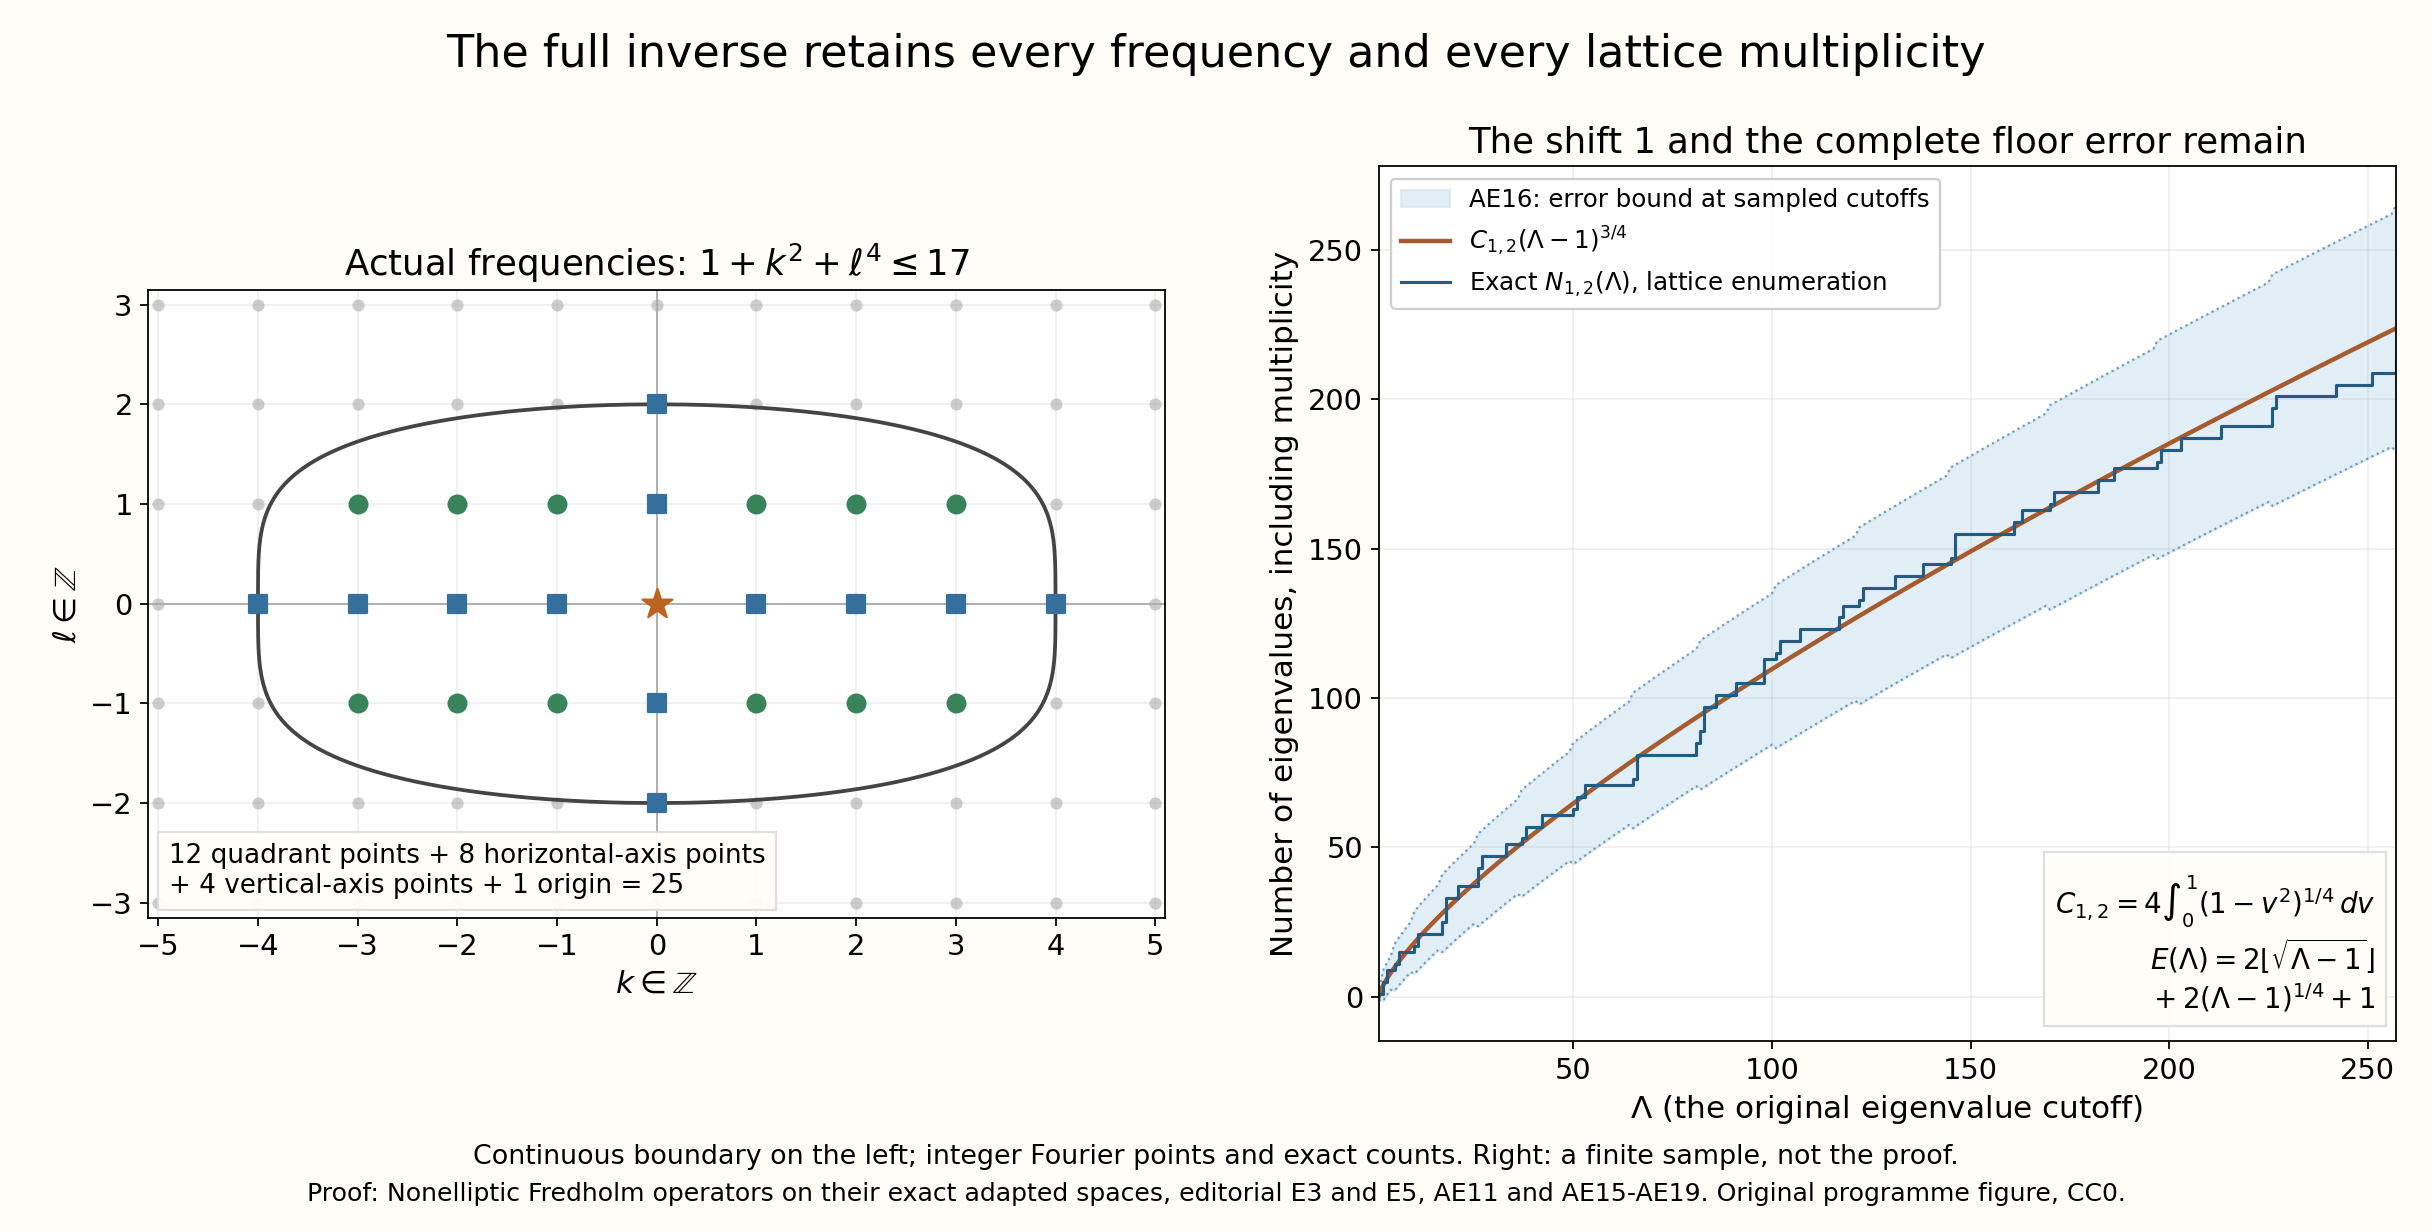
\includegraphics[keepaspectratio,alt={The original lattice spectrum and its exact shifted counting bound}]{../figures/adapted-exact-spectrum-264.png}}
\caption{The original lattice spectrum and its exact shifted counting
bound}
\end{figure}

The left panel is the actual integer-frequency spectrum below
\(\Lambda=17\) for the original \(r=1,m=2\) operator; its boundary is
the continuous section \(1+k^2+\ell^4=17\), not an additional frequency
set. The origin and both axes are counted separately in (AE15). The
right panel compares the exact staircase with
\(C_{1,2}(\Lambda-1)^{3/4}\) and the proved full error bound in (AE16),
including the shift, the floor, and the final one. The graph is a finite
numerical sample of that proved inequality, whose proof is E5. The
reproducible source is
\href{../figures/adapted-exact-spectrum-264.py}{adapted-exact-spectrum-264.py}.
These figures and arguments are original programme derivations dedicated
to the public domain under the lesson's CC0 dedication; no external
proof or novelty claim is being substituted for the complete
calculation.

\subsubsection{E6. Distributions defined only on the open
set}\label{e6.-distributions-defined-only-on-the-open-set}

The theorem (AH25) was stated for a distribution on the entire torus.
Its conclusion also holds for a distribution defined only on the given
open set. We prove the precise extension and restriction maps, using the
same operator \(P_{r,m}=I+(-1)^r\partial_x^{2r}+(-1)^m\partial_y^{2m}\)
with the original integers \(1\leq r<m\). The derivatives and the
measure \(dx\,dy\) are the original period-\(2\pi\) torus ones.

Write \(\mathcal D(U)=C_c^\infty(U)\). Its distributions are linear
functionals continuous on each space \(\mathcal D_K(U)\) of tests
supported in a fixed compact \(K\subset U\), with seminorms
\(\max_{|\alpha|\leq N}\|\partial^\alpha\psi\|_\infty\). This is the
distribution convention already used in E1--E2. Restriction to a smaller
open set means evaluation on the zero extension of its compactly
supported tests; that zero extension is smooth because its support is
contained in the smaller open set.

Fix a point \(z_0=(x_0,y_0)\in U\). Choose \(\varepsilon>0\) so that the
closed coordinate ball of radius \(2\varepsilon\) about \(z_0\) is
contained in a coordinate chart inside \(U\). Let \(W\) be the ball of
radius \(\varepsilon/2\). There is a smooth cutoff \(\eta\) supported in
that closed larger ball and equal to one on the ball of radius
\(\varepsilon\). Here is an explicit construction that also fixes its
support. Put \(\zeta(s)=e^{-1/s}\) for \(s>0\) and \(\zeta(s)=0\) for
\(s\leq0\). Each derivative on the positive half-line is an exponential
times a polynomial in \(1/s\), which tends to zero as \(s\downarrow0\):
indeed \(e^t\geq t^{M+1}/(M+1)!\) implies \(t^Me^{-t}\leq(M+1)!/t\to0\).
Thus \(\zeta\) is smooth. In the chosen chart set
\(s=((x-x_0)^2+(y-y_0)^2)/\varepsilon^2\) and
\(\eta=\zeta(4-s)/(\zeta(4-s)+\zeta(s-1))\), extending it by zero
outside the chart. The denominator is positive everywhere in the chart:
its two summands could both vanish only if \(s\geq4\) and \(s\leq1\).
This cutoff is one for \(s\leq1\), zero for \(s\geq4\), and its zero
extension is smooth. In particular it is one on a neighbourhood of
\(\overline W\). Let \(K=\operatorname{supp}\eta\subset U\).

For \(w\in\mathcal D'(U)\) define an actual distribution on the whole
torus by \[
 E_\eta:\mathcal D'(U)\longrightarrow\mathcal D'(\mathbb T^2),
 \qquad (E_\eta w)(\varphi)=w\bigl((\eta\varphi)|_U\bigr),
 \qquad \varphi\in C^\infty(\mathbb T^2).
 \tag{AE21}
\] For the fixed compact \(K\), continuity of \(w\) supplies a finite
order \(N\) and \(C\geq0\) with \(|w(\psi)|\leq C\max_{|\alpha|\leq N}
\|\partial^\alpha\psi\|_\infty\) for \(\psi\in\mathcal D_K(U)\). The
full product rule gives \[
 |(E_\eta w)(\varphi)|
 \leq C\max_{|\alpha|\leq N}
 \sum_{\beta\leq\alpha}\binom{\alpha}{\beta}
 \|\partial^{\alpha-\beta}\eta\|_\infty
 \|\partial^\beta\varphi\|_\infty.
 \tag{AE22}
\] Every summand and cutoff derivative is retained. This is a finite
continuous seminorm bound on torus tests and proves that (AE21) has its
stated codomain. The map is linear. With the topology of convergence on
every fixed test in each distribution space it is continuous, since
evaluation of its image on \(\varphi\) is exactly evaluation of its
input on the fixed test \((\eta\varphi)|_U\).

For any \(\psi\in\mathcal D(W)\) we have \(\eta\psi=\psi\). The formal
transpose of this particular operator is itself: each derivative has
even order, and its coefficient remains respectively
\(1,(-1)^r,(-1)^m\). Moreover
\(\operatorname{supp}(P_{r,m}\psi)\subset\operatorname{supp}\psi\), so
\(\eta P_{r,m}\psi=P_{r,m}\psi\). Consequently the exact restriction
identities, with all domains shown, are \[
 \begin{aligned}
 \operatorname{res}_W E_\eta w&=\operatorname{res}_W w
          &&\text{in }\mathcal D'(W),\\
 \operatorname{res}_W(P_{r,m}E_\eta w)
      &=P_{r,m}|_W(\operatorname{res}_W w)
          &&\text{in }\mathcal D'(W).
 \end{aligned}
 \tag{AE23}
\] To verify the second line on a test rather than suppress a cutoff
contribution, its left-hand side is
\(w((\eta P_{r,m}\psi)|_U)=w((P_{r,m}\psi)|_U)\). The right-hand side
has exactly that value by the definition of the local distributional
derivative. The equality is after restriction to \(W\), where the cutoff
is identically one; no global commutation of \(P_{r,m}\) with
multiplication by \(\eta\) is asserted.

Suppose now that \(P_{r,m}w\) is represented by a smooth function on
\(U\). By (AE23), \(P_{r,m}E_\eta w\) is smooth on \(W\). Apply the
already proved theorem (AH25) to the global distribution \(E_\eta w\)
and the open set \(W\). It gives a smooth representative there. The
first line of (AE23) identifies that representative with \(w|_W\). The
balls \(W\) obtained for all points cover \(U\), so \(w\) is smooth on
\(U\).

For completeness, the local smooth representatives agree on overlaps. If
their difference had a nonzero value at a point, multiplication by a
fixed complex unit would make its real part positive on a smaller ball.
A nonnegative, nonzero smooth test supported in that ball would then
give a nonzero distributional value, contradicting equality of the
restrictions. They therefore patch to a unique smooth function. It
represents the original distribution on every test: a compact test
support has a finite cover by the balls above, and smaller cutoff balls
give smooth functions \(\chi_i\geq0\) supported in those balls with
\(\sum_i\chi_i>0\) near that support. Decompose the test there as
\(\sum_i\chi_i\psi/(\sum_j\chi_j)\), with zero extensions where the
denominator is not needed. Each summand has compact support in its ball
and has the corresponding representative. Their sum gives the original
pairing with the function using \(dx\,dy\).

Conversely a smooth \(w\) has smooth \(P_{r,m}w\) by the displayed
finite differential formula. Thus for every open \(U\subset\mathbb T^2\)
and every \(w\in\mathcal D'(U)\), smoothness of \(P_{r,m}w\) on \(U\) is
equivalent to smoothness of \(w\) there. The empty set has only its zero
distribution, so is included. The argument also applies when \(U\) is
the entire torus; no extension outside the torus is used. This
strengthens the domain of (AH25) and leaves the distinct adapted
Fredholm and ordinary Sobolev assertions unchanged.

The local-kernel figure now labels the input \((1-\chi)f\), whose
support is separated from \(V\), and its smooth output \(Q((1-\chi)f)\),
whose support may meet \(V\). The exact receiving map and counterexample
proving this distinction are in E2. Its footer also displays (AE21) and
the restricted operator identity (AE23), which allow the same local
argument for distributions initially defined only on \(U\). These are
original programme proofs, with the same CC0 dedication and without an
external proof citation.

\end{document}
